%%%%%%%%%%%%%%%%%%%%%%%%%%
% USFD Academic Report Template
% Prof. Roger K. Moore
% University of Sheffield
% 30 July 2018
%%%%%%%%%%%%%%%%%%%%%%%%%%


\documentclass[11pt,oneside]{book}
\usepackage[margin=1.2in]{geometry}
\usepackage[toc,page]{appendix}
\usepackage{graphicx}
\usepackage{listings}

\usepackage{longtable}
\usepackage{natbib}
\usepackage{lipsum}
\usepackage{caption}
\usepackage{amsmath}
\usepackage{subcaption}
\usepackage[colorinlistoftodos]{todonotes}
\usepackage[colorlinks=true, allcolors=blue]{hyperref}
\usepackage{float}
\lstset{language=Python}          % Set your language (you can change the language for each code-block optionally)
\definecolor{codegreen}{rgb}{0,0.6,0}
\definecolor{codegray}{rgb}{0.5,0.5,0.5}
\definecolor{codepurple}{rgb}{0.58,0,0.82}
\definecolor{backcolour}{rgb}{0.95,0.95,0.92}
 
\lstdefinestyle{mystyle}{
    backgroundcolor=\color{backcolour},   
    commentstyle=\color{codegreen},
    keywordstyle=\color{magenta},
    numberstyle=\tiny\color{codegray},
    stringstyle=\color{codepurple},
    basicstyle=\footnotesize,
    breakatwhitespace=false,         
    breaklines=true,                 
    captionpos=b,                    
    keepspaces=true,                 
    numbers=left,                    
    numbersep=5pt,                  
    showspaces=false,                
    showstringspaces=false,
    showtabs=false,                  
    tabsize=2
}
 
\lstset{style=mystyle}
\begin{document}

\captionsetup[figure]{margin=1.5cm,font=small,labelfont={bf},name={Figure},labelsep=colon,textfont={it}}
\captionsetup[table]{margin=1.5cm,font=small,labelfont={bf},name={Table},labelsep=colon,textfont={it}}
\setlipsumdefault{1}

\frontmatter

\begin{titlepage}


% -------------------------------------------------------------------
% You need to edit the details here
% -------------------------------------------------------------------

\begin{center}
{\LARGE University of Sheffield}\\[1.5cm]
\linespread{1.2}\huge {\bfseries Comparison of quadruped locomotion using Coupled Oscillators to the Dynamic Similarity Hypothesis}\\[1.5cm]
\linespread{1}

\includegraphics[width=5cm]{images/tuoslogo.png}\\[1cm]
{\Large Damian Bemben}\\[1cm]
{\large \emph{Supervisor:} Roger K Moore}\\[1cm] % if applicable
\large A report submitted in partial fulfilment of the requirements\\ for the degree of \textbf{Computer Science with a Year in Industry MComp} 
 in Computer Science\\[0.3cm] 
\textit{in the}\\[0.3cm]
Department of Computer Science\\[1cm]
\today
\end{center}
\end{titlepage}


% -------------------------------------------------------------------
% Declaration
% -------------------------------------------------------------------

\newpage
\section*{\Large Declaration}

All sentences or passages quoted in this document from other people's work have been specifically acknowledged by clear cross-referencing to author, work and page(s).  Any illustrations that are not the work of the author of this report have been used with the explicit permission of the originator and are specifically acknowledged.  I understand that failure to do this amounts to plagiarism and will be considered grounds for failure.\\[1cm]

\noindent Name: Damian Bemben\\[1mm]
\rule[1em]{25em}{0.5pt}

\noindent Signature:\\[1mm]
\rule[1em]{25em}{0.5pt}

\noindent Date:\\[1mm]
\rule[1em]{25em}{0.5pt}


% -------------------------------------------------------------------
% Abstract
% -------------------------------------------------------------------

\chapter*{\Large \center Abstract}

% Guidance of how to write an abstract/summary provided by Nature: https://cbs.umn.edu/sites/cbs.umn.edu/files/public/downloads/Annotated_Nature_abstract.pdf

The Dynamic Similarity hypothesis states that different mammals will exhibit dynamically similar movement when travelling at a velocity that grants them equal Froude Numbers, a calculation based on measurements of an animal's height, which indicates the gait an animal will be performing. Gaits can be generated for a quadruped robot through the replication of Central Pattern Generators (biological neural circuits in animals that produce rhythmic outputs) using groups of coupled non-linear oscillators producing periodic oscillatory movement, with coupling performed through the use of neuronal links between oscillators. Other methods used to replicate quadruped movement tend to either be limited to common species due to difficulties in collecting training data for wild animals or if done through other mathematical methods, do not compare themselves directly to their real life counterparts. Here we show that simulated gaits using coupled Van der Pol oscillators adhere to the dynamic similarity hypothesis, with over 70\%  of successful walking gaits exhibiting ranges of Froude number found in living mammals. These results demonstrate that although simulated gaits can reach larger Froude numbers (and hence faster velocities) than evolutionary values, Froude number can be used as a valid guideline for successful gait generation. This research provides a starting point for investigating and comparing simulated gaits to living mammals. Furthermore, this is the first open-source implementation of coupled oscillators as Central Pattern Generators, and as such could be used for more sophisticated research into the design of quadruped gaits in the future. 

% We will show how natural gaits can be generated for a quadruped robot through replication of a central pattern generator by the use of Coupled Van der Pol Oscillators and compare these values to those found for real mammals in the Dynamic Similarity Hypothesis. By investigating effects on In addition to this, we find that combinations of parameters who's values reach above Froude numbers seen in evolutionary principles produce far more variation, and are more likely to produce unstable and ineffective movement than combinations in which more values lie between acceptable values.

% These results show that provide a starting point for the development of realistic mammal gaits, and a method of comparing robotic gaits to real counterparts. This could have potential uses in the initial stages of quadruped gait design, as  `

% 
% Acknowledgments

\input{sections/acknowl.tex}

% -------------------------------------------------------------------
% Contents, list of figures, list of tables
% -------------------------------------------------------------------

\tableofcontents
\listoffigures
\listoftables


% -------------------------------------------------------------------
% Main sections (as required)
% -------------------------------------------------------------------

\mainmatter

\chapter{Introduction}
% Animal movement has been replicated

In nature, rhythmic movements such as walking, breathing or chewing are controlled by neural networks providing co-ordinated patterns for actions. These networks are more commonly referred to as Central Pattern Generators (CPGs) \citep{MarderEveBucher2001}. This dissertation will focus  on the use of CPGs in the creation of animal locomotion. One way to represent CPGs is through the use of coupled non-linear oscillators that generate rhythmic patterns, non-linear referring to the periodic signal of the oscillator not moving constantly at the same rate. A single non-linear oscillator can represent the rhythmic movement for a single limb of an animal. Gaits can  be replicated by creating coupling in-between oscillators. Coupling provides a method of replicating gaits by the creation of hard-wired links between oscillator values that create different rhythmic patterns, and so can replicate actions such as walking, trotting or running. 

Animal movement has been shown to follow certain patterns - many mammals share similar styles of walks, trots and other gaits. Dynamic Similarity is a hypothesis that claims two different mammals travelling with similar Froude Numbers (a value derived from simple measurements about an animal) \footnote{Froude Number may refer to other physical systems \citep{Pratt2008}. All mentions of a Froude Number in this dissertation refer to the Froude Value described in \cite{Alexander1983}} will use the same gaits \citep{Alexander1983}. Froude Number can be represented by equation \ref{froude:equation1}, where v represents velocity, g represents gravitational acceleration and h represents height at the hip.

\begin{equation}
F = v^2/gh
\label{froude:equation1}
\end{equation}

Although this hypothesis was only applied to living mammals, there have since been many examples of quadruped robots designed to move in a similar fashion to living mammals, from MiT's Cheetah \citep{Wensing2017} to  Boston Dynamic's Big Dog \citep{Raibert2008}. This leads to the hypothesis that a quadruped robot performing generated gaits will also need to adhere to the Dynamic Similarity hypothesis.

Despite the large number of robotic quadrupeds designed to perform like mammals, There exists little research on whether the concept of Dynamic Similarity would still apply to a robotic quadruped. This research aims to examine and compare the similarities and differences between a simulated robotic quadruped and information on animals found in the Dynamic Similarity Hypothesis.
% We i this through the comparison of a simple robot
% we could in turn estimate parameters such as speed and time period the animal should be travelling at. This could provide an important initial estimate on what the parameters of a given Central Pattern Generator, to maintain both balance, and reduce cost of travel \cite{Yong2005}. Currently, a large amount of literature uses parameters either from parameter tweaking, or estimates. 

\section{Aims and Objectives}
This dissertation will implement a CPG into a physics based simulation, through the use of a robot model based on a real counterpart. Although the Dynamic Similarity hypothesis has been applied to comparing human and dog gaits \citep{Gan2018a}, a direct comparison has not yet been made between quadruped robots and living mammals. 

An evaluation will be made as to whether these values are within the confines found in \cite{Alexander1983}. This will be done through calculating the Froude Number for a simulated quadruped and comparing it against Froude Number values found in the Dynamic Similarity Hypothesis.

This aims to find out if the Dynamic Similarity Hypothesis still holds for a simulated quadruped using coupled oscillators for its CPG. This  aims to showcase that the Dynamic Similarity hypothesis can be applied to real quadruped robots in the future. This aims to showcase a potential method of finding parameters for quadruped robots in future research, as well as a potential rubric for investigating robotic gaits.

% , as given the height of an arbitrary robot, we can in turn find the range of velocities that different gaits should be performing at.

\section{Overview}
This dissertation will begin with a literature survey describing in  detail the concept of Dynamic Similarity followed by an overview of gait generation methods. A justification will be made for why coupled Van der Pol oscillators where decided to be the method of gait generation followed by a detailed description of how this method was implemented. An evaluation will be made for which robot environment is most appropriate for creating a comparison. 

Testing criteria used to find appropriate ranges of parameters for testing will be described, along with a description of the testing environment for the final findings. The model made will be compared to values found in the Dynamic Similarity hypothesis, and show whether gait generation using a coupled oscillator as a Central Pattern Generator produces gaits similar to that seen in actual mammals. There will be a discussion of the findings, detailing the successes and failures of the project.This will be followed with  further work that could be done with the model created.

\section{Relationship Between Project and Degree Program}
The work done in this dissertation provide close links with modules such as Natural Systems and Adaptive Intelligence. This has proven advantageous, in that both of these modules contain assignments based on writing academic reports. Additionally, the work on derivatives in natural systems provided a more in depth understanding of how the van der pol oscillator worked, giving a clearer understanding of derivative solutions and equations, and the implementation of them in Python. However, a large amount of the work done in this dissertation has not been part of the computer science curriculum, especially proper statistics design and T-tests for similarity, this required a large amount of research on appropriate tests to run.

\chapter{Literature Survey}
This survey has been broken down into two main sections: Dynamic Similarity which will detail current research performed by \cite{Alexander1983} along with an explanation on potential shortcoming of the research and Gait Generation, which will explain in more detail the concept of a Central Pattern Generator before focusing on potential methods of gait generation found for this project.
\section{Dynamic Similarity}


The concept of Dynamic Similarity is mentioned in \cite{Skrba2010}, which describes potential quadruped animation methods, it is however only used as a guideline for animators to follow. Additionally, \cite{Skrba2010} mentions the difficulty in current methods of  gaits animation and generation. Standard motion capture is shown to be difficult with wild animals, with the data being specific to the animal trained on, making it difficult to extend on other mammals. This is seen with \cite{Alexander1983} attempting to find gait values for wild Coypu, which provide far different results to the rest of the trends seen, due to the Coypu acting in a "nervous manner". 
% Additionally, motion capture data will not be gathered for this dissertation, reducing the risk of data captured being "very specific to a particular animal and its movements"
% As this dissertation aims to use the Dynamic Similarity hypothesis as not a guideline, this should provide a more generic way of creating animal gaits. 
\cite{Alexander1983}contains a large amount of information on how the Froude number is shown to affect separate parts of mammals, as graph data is shown for Phase Relationships, Relative Stride Lengths and Forces on The Feet. 

This leads to the assumption that given the height of the animal as well as a Froude Number to represent gait, the speed of a certain gait can therefore be inferred. Dynamic Similarity is most apparent in Cursorial Mammals, which  exhibit similar relative stride lengths at the same Froude Numbers Equations for stride length against Froude number have been found in Alexander's research to take the following form, for walking gaits, a =, with b=, with faster gaits taking the following form. 


\cite{Alexander1983} makes an important distinction between non-cursorial and cursorial mammals with the hypothesis remaining accurate for examining only cursorial or non-cursorial mammals, but becoming inaccurate when considering both. Cursorial Mammals are typically referred to as animals that have adapted to run, although \cite{Garland1993} states that this not a strong enough metric for whether a mammal is cursorial. \cite{Stein1997} defines cursorial mammals as having limbs in the parasaggital plane. The saggital plane divides the body into two halves vertically, with the parasaggital plane referring to anywhere parallel to this plane. A visual example of the parasaggital plane in a cursorial mammal can be seen in \ref{fig:parasaggital}. 
 
\begin{figure}
    \centering
    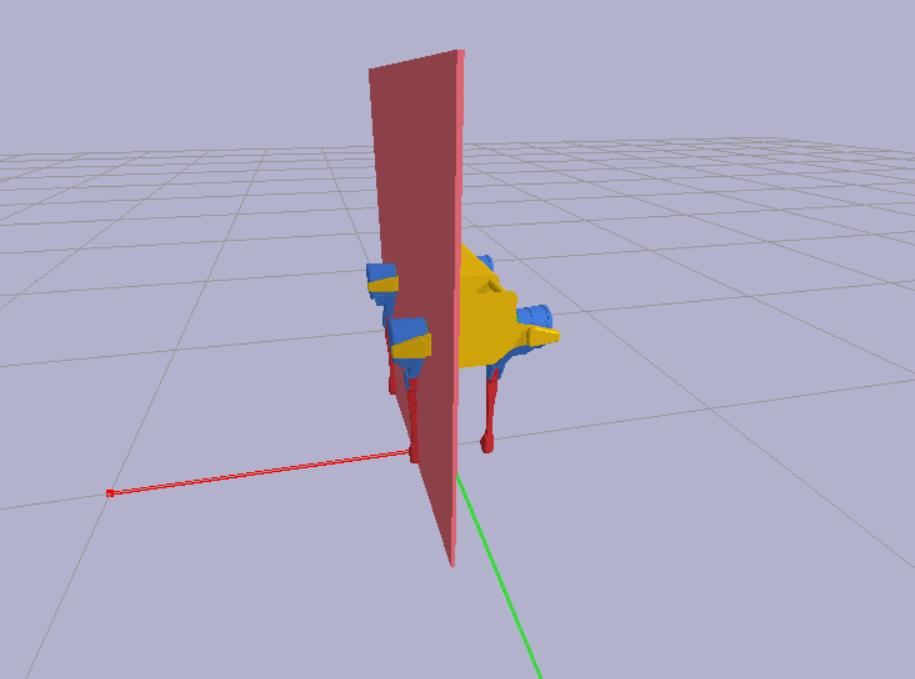
\includegraphics[width=0.4\textwidth]{figures/parasaggital.png}
    \caption{Diagram of robot parasaggital plane, indicated by the red square}
    \label{fig:parasaggital}
\end{figure}

The difference in Dynamic Similarity between cursorial and non-cursorial mammals is thought to be due to non-cursorial mammals having a far longer relative stride length than cursorial mammals. \cite{Gan2018a} investigates Dynamic Similarity between bipeds and quadrupeds, which further showcase the limitations of this Hypothesis, as there only exists similarity between quadrupeds and bipeds in  specific scenarios such as bounding. This in turn limits the Dynamic Similarity Hypothesis to cursorial mammals.


In order to showcase similarity between cursorial gaits \cite{Alexander1983} defined two separate subsets: walking, which occurs at Froude numbers below 0.4 and faster gaits, which occur above 0.4. Animals performing gaits have been described the equation \ref{froude:equation}, with x representing values of relative stride lengths. \cite{Carr2016} defines Stride Length as the distance from one step to the next step of the same leg. 

\begin{equation}
x = a*(v^2/gh)^b
\label{froude:equation}
\end{equation}

Parameter a, exponent b, deviations and froude number limits are defined by table \ref{table:froude}. As this data was gathered in 1983, the testing methods have a large margin of error.

\begin{table}[width=15cm]
\begin{tabular}{lllll}
Gait         & Factor a & Exponent b   & Standard Deviation & Froude Number Limits \\
Cursorial Walking      & 2.4      & 0.34 +- 0.1  & 1.16                      & F \textless 0.4       \\
Cursorial Faster Gaits & 1.9      & 0.40 +- 0.03 & 1.14                      & F \textgreater 0.4    \\
                               &          &              &                           &                      
\end{tabular}
\caption{Table of Froude number values}
\label{table:froude}
\end{table}

A similar concept to Dynamic Similarity although not specific to Animal Locomotion has been developed by \citep{Reveret2009} who uses expert animators in order to create morph-able quadruped skeletons. As a large amount of data is based on animator design, it may not be scientifically suitable, but it does show the potential of creating adaptable mammalian quadruped skeletons, and as the skeleton allows for morphing based on geometric measurements, a similar method could be used in order to build a robotic model. 

\section{Gait Generation}

A Central Pattern Generator is a biological neural network that provides an animal with it's natural walking rhythm, however it is also used in other actions that require periodic movements, such as chewing and breathing.  \cite{MarderEveBucher2001} shows how central pattern generators work in living mammals by investigating the movement of a locust's wings. This in turn finds that the mechanisms of rhythm generation are created by the use of neurons that produce periodic signals to couple, and produce more complex rhythmic patterns, such as walking. There are various methods for the recreation of Central Pattern Generators. 

\citep{Kruger2014} provides multiple methods of gait reconstruction, and evaluates their success rate. Although focused on retrieval from motion capture data, which is not the primary focus of this project, it highlights the primary issues with gathering motion capture data and using it to infer gaits, as although the experiments shown in \cite{Kruger2014} are successful, there does not exist a large motion capture database. This correlates with information gathered from \cite{Skrba2010}, which claims that the major issue with gathering motion capture data is that wild animals are difficult to gather a large dataset for.

\cite{Geijtenbeek2013} produces a method of locomotion for different types of bipeds through the implementation of a musco-skeletal model. Although this sort of model would not be possible to directly be implemented into a robotic design due to the high complexity of the model, and it does not involve a neuronal central pattern generator (instead using a finite state machine to decide method constriction and expansion), it showcases the possibility of a locomotion system being adaptable to multiple models. One of the methods that \cite{Geijtenbeek2013} uses in order to optimise the gaits is through the use of a Covariance Matrix Adaptation \cite{Hansen2016}, an evolutionary principle that is particularly effective in small population sizes, and so would be effective in the small populations used in \cite{Geijtenbeek2013}. 

An interesting implementation of recreating quadruped gaits is shown in \cite{Zhang2018}, who proposes using Mode-Adaptive Neural Networks. It is used to create a variety of complex movements such as obstacle navigation, jumping and gait correction. The focus of \cite{Zhang2018} was in creating realistic animations, and as they are not applied directly to the design of a robot, the methods seen may not apply to a real model of a robot. Additionally, \cite{Zhang2018} gathers data based from Dog motion capture data, which means that the design of the network is focused on data from dog gaits, and would be unable to easily translate to other animals. 

\cite{Fukuoka2015} implements gait generation  through the use of a CPG and applies leg loading feedback to assist in navigation of uneven surfaces. This design applies to normal gaits as well as converting between walking and faster gaits. The design of this 

A frequently used method has been through the use of non-conservative oscillators. \cite{Rutishauser2008} implements a central pattern generator through the use of a derivative equation, with oscillators being coupled together through the use of a 4x4 size matrix. This produces a stable walking gait, however comes into trouble when trying to replicate a faster gait pace. However, \cite{Rutishauser2008} appears to find a walking gait far more stable than that of a trot, with a trot performing far less stable and slower gaits, and actually being far more unstable at faster speeds. 

Van der Pol oscillators have shown to be extremely common in the replication of central pattern generators, being used successfully in \cite{Low2006} for the replication of Jellyfish Locomotion. A Van der Pol Oscillator is a non-linear oscillator that can be described by a second-order differential equation \citep{Barbosa2007}. The equation of a normal Van der Pol oscillator is described by equation \ref{vanderpol:pure}
\begin{equation}
\ddot{x} + \alpha(x^2 - 1)\dot{x} + x = 0
\label{vanderpol:pure}
\end{equation}

\cite{Collins1994} investigates multiple different non-linear oscillators for the replication of quadruped gaits, one of the types of non-linear oscillators that stands out is the Van der Pol oscillator. \cite{Collins1994} used coupled Van der Pol generators to recreate quadruped gaits mathematically. Although this is not implemented in a real model, it appears to shows how the generator can create transitions from different gaits, and react to real-time changes in coupling parameters. The slightly modified Van der Pol oscillator in \cite{Collins1994} is described by equation \ref{vanderpol:mod}.

\begin{equation}
\ddot{x} + \mu(x^2 - p^2)\dot{x} + g^2x = 0
\label{vanderpol:mod}
\end{equation}

Where mu, p and g are free parameters. This allows more direct control over the period and shape of the Van der Pol oscillator.

\cite{Yocono2015} describes the dynamics of a van der pol oscillator in more detail, and provides an implementation of a Van der Pol oscillator in python, showcasing the use of the oscillator in hair cell auditory responses. However, \cite{Yocono2015} does not implement coupling of any form for this. \cite{Yocono2015} uses a modified Van der Pol oscillator as seen in equation \ref{vanderpol:mod}, which suggests that this modified form is common.

\cite{Liu2009} provides an implementation of a Van der Pol oscillator in a robotic quadruped. For this implementation, $x^2$ and $p^2$ are switched around, and the equation is put into a two-dimensional form for ease of implementation. This results in \ref{vanderpol:twod} 


\begin{equation}
\dot{x} = y,   \dot{y} = \alpha(p^2 - x^2)y - w^2x
\label{vanderpol:twod}
\end{equation}

This equation is shown to produce valid walking, trotting, bounding and pacing gaits. However, only the success of the implementation is measured, with no work done on improving efficiency or energy expenditure. Additionally, the parameters used for this paper are arbitrary. \cite{Liu2019} shows that implementation of a van Der Pol oscillator into a robot quadruped can produce successful gaits and do it through the use of a relatively simple differential equation. Coupling in \cite{Liu2009} is performed in a similar way to the coupling found in \cite{Collins1994}. This is done through the use of a 4x4 matrix of values, with a coupling parameter for each limb, with the equation for coupling oscillator a to oscillator i can be seen in equation \ref{vanderpol:coupling}

\begin{equation}
x_{ai} = x_{i} + \sum_{j}{\lambda_{ij}x_{j}}
\label{vanderpol:coupling}
\end{equation}

Due to the similarity between the coupling found in \cite{Collins1994} and \cite{Liu2009}, this appears to be a common method of coupling between oscillators. One of the interesting differences is that although both oscillator equations are almost identical, the coupling matrices for \cite{Collins1994} and \cite{Liu2009} are different. This could be due to different parameters used in \cite{Collins1994} due to them not having an actual implementation in a working robot.
% balancing\citep{Meng2015}
A potential issue in gait generation for a quadruped robot is stability. \cite{Meng2015} provides a method of balancing through the use of.  \cite{PrescottTonyJLeporaNathanFVerschure2018}, which shows how the centre of mass is guided via gravity during a horse trot. By following optimal speeds at certain gaits, this could potentially to allow the Centre Of Mass of the system to 'float' when encountered with small obstacles, essentially dealing with small issues

% \citep{PrescottTonyJLeporaNathanFVerschure2018}
% By adhering to the evolutionary principle, this could provide a method in which some natural stability might be observed. This can be seen in
% \begin{equation}
% \ddot{x} + \alpha(x^2 - 1)\dot{x} + x = 0
% \label{vanderpol:pure}
% \end{equation}

% \begin{equation}
% \ddot{x} + \alpha(x^2 - 1)\dot{x} + x = 0
% \label{vanderpol:pure}
% \end{equation}


% \begin{equation}
% \ddot{x} + \alpha(x^2 - 1)\dot{x} + x = 0
% \label{vanderpol:pure}
% \end{equation}

% \begin{equation}
% M = \frac{1}{T}\sum_{t=1}^{T} e(t) / \max_{t}[e(t)]
% \label{eq:equation}
% \end{equation}

%   % Replace with your text

% This is shown in Equation \ref{eq:equation} and is repeated here $M = \frac{1}{T}\sum_{t=1}^{T} e(t) / \max_{t}[e(t)]$.


% \section{Evaluation}

% \begin{figure}[ht]
% 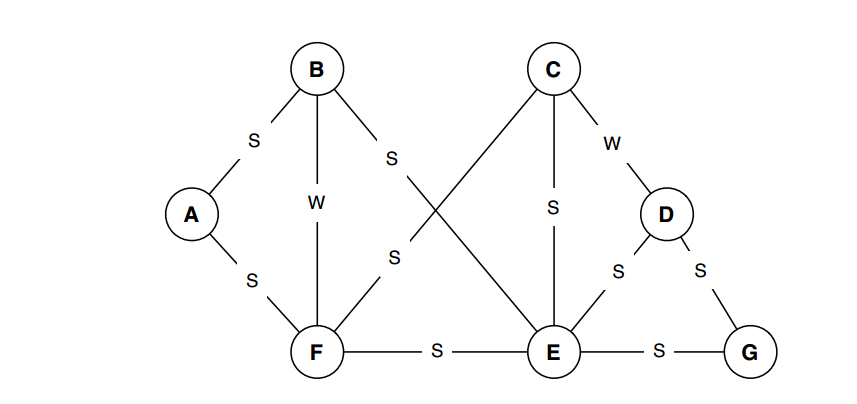
\includegraphics[width=15cm]{figures/figure1.png}
% \caption{A simple figure in \LaTeX. Reproduced from http://tinyurl.com/nqtrlj5 with the permission of the copyright owner.}
% \label{fig:graph}
% \end{figure}

  % Replace with your text

% See Figure \ref{fig:graph}.


  % Replace with your text

% \begin{table}[ht]
% \center
% \begin{tabular}{cc|c}
% A & B & A XOR B\\
% \hline
% 0 & 0 & 0\\
% 0 & 1 & 1\\
% 1 & 0 & 1\\
% 1 & 1 & 3\\
% \end{tabular}
% \caption{A simple table in \LaTeX.}
% \label{tab:xor}
% \end{table}

  % Replace with your text

% This is shown in Table \ref{tab:xor}.


\section{Summary}
Through this review, many valid methods where found for the recreation of a living mammals Central Pattern Generator. However, very few of the current methods seen use the concept of Dynamic Similarity to a large extent.

The research found in \cite{Alexander1983} is slightly out-dated, especially with the methods of data collection, such as the use of extrapolation over distance for certain African mammals. However, this does not make the hypothesis invalid, as it has shown to apply for a wide range of animals tested.

Although there are a wide range of methods for creating Central Pattern Generators, many use methods that would not be directly applicable to a real robot, such as the recreation of muscular skeletal systems in \cite{Geijtenbeek2013} or would be outside the scope of the Dissertation. The use of coupled non-linear oscillators, due to it's relative simplicity as well as effectiveness in generating robotic gaits seems to be appropriate in scope, and would be able to produce valid gaits.

Although various models have been investigated on how to generate realistic quadruped gaits, a model has not been found that compares against results found in Dynamic Similarity. This could be especially useful for the Van der Pol oscillator due to it's effectiveness in modelling other natural systems.

% \begin{figure}
%     \centering
%     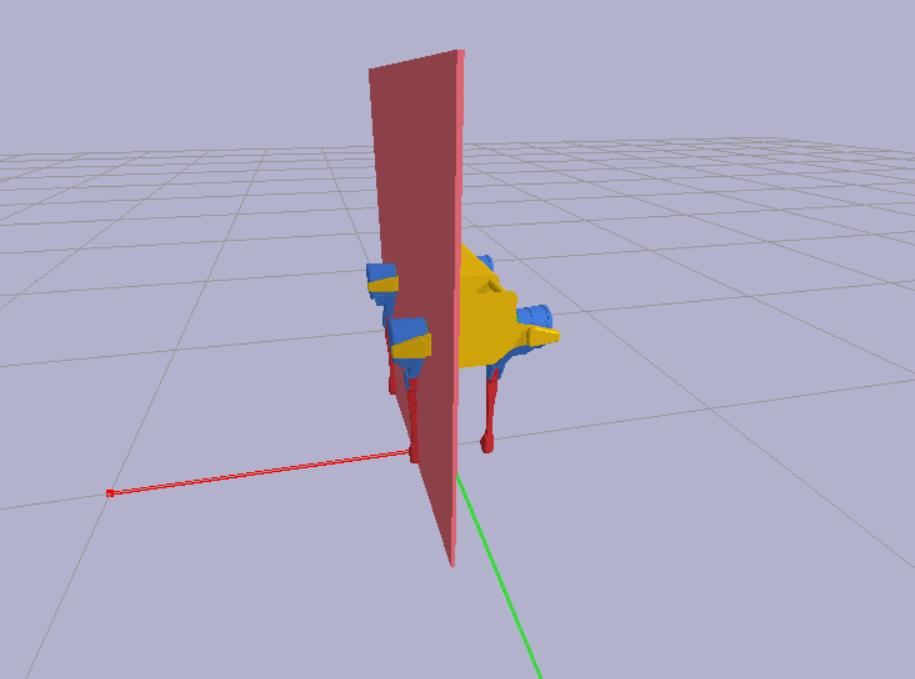
\includegraphics[width=0.8\textwidth]{figures/parasaggital.png}
%     \caption{Diagram of robot planes, the red square indicates the robots Parasaggital plane.}
%     \label{fig:vanderpol}
% \end{figure}

% There are many different available options of oscillator, from the Stein neuronal model, which is typically used to simulate a neuron itself. In this paper, we wish to focus on the investigation of the van der pol oscillator, which takes the following second-order nonlinear differential equation, this equation can be seen in \ref{vanderpol:pure}.


% Certain gaits can be shown mathematically, for example, \cite{} describes the following gaits numerically, with phase difference between gaits being labelled. 
% \begin{figure}
%     \centering
%     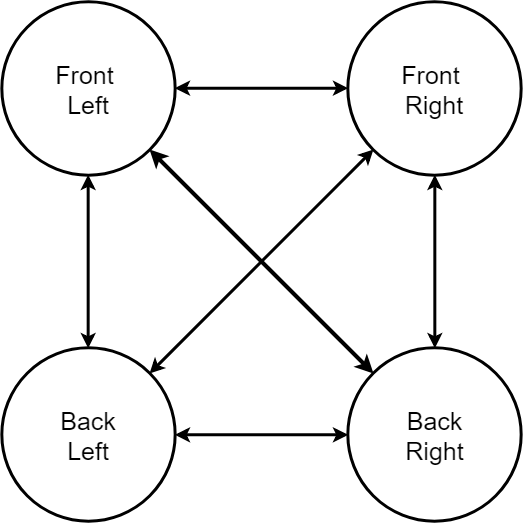
\includegraphics[width=0.3\textwidth]{figures/coupling.png}
%     \caption{Diagram of coupling combinations.}
%     \label{fig:coupling}
% \end{figure}

\chapter{Methodology}


\section{Requirements}
% This should state, in a more detailed way, the objectives of the project by requirement and the analysis should break the problem down into manageable steps. There may be more than one suitable approach; the analysis may cover more of the area than is finally implemented. Testing and evaluation should be given due consideration. It is important that you state how you will evaluate your work. For a design project it is appropriate to consider testing at the same time as specification.

The main requirement of this dissertation is the comparison between the Dynamic Similarity hypothesis and a simulated model, in order to establish whether a simulated gait still conforms to the values seen in the Dynamic Similarity hypothesis. For this to succeed, a valid robotic environment is required, this could take the form of a real quadruped robot or a physics simulation of a quadruped robot. If a physics environment is used, the robotic model must be based on a real life counterpart to allow for direct comparisons between real examples, as it may skew the results of the investigation to use a unrealistic model. 

This will indicate that the mathematical methods of generating gaits used in this dissertation would be valid for a real robot and that robots follow the rules of Dynamic Similarity outlined in \cite{Alexander1983}.

Although evaluating a range of different gaits is optional, it would be useful to investigate whether the same difference between cursorial walking and faster gaits is seen, as this would further prove the results. This could be done through the results found in \ref{table:froude}, through investigating Stride Length.

% useful to see whether the same issues occur as found in \cite{Rutishauser2008}, wherein faster gaits broke down more easily and produced slower movement than a walking gait.
 

\section{Analysis}
In order to break down the problem into easily manageable steps, The analysis stage has been separated into the creation of a Central Pattern Generator, the implementation of the Central Pattern Generator in a robotic environment. Additionally, a large portion of the analysis will include an analysis on the  evaluation of the gait against the Dynamic Similarity Hypothesis.

\subsection{Central Pattern Generator}
Initially, this dissertation wishes to focus on the CPG design, due to it being an integral part of the project. Additionally, many many of the methods found create the CPG first, followed by the implementation of the CPG in a robotic environment. 

There is the possibility of designing the motor actions separately, and use an evolutionary technique similar to the muscular skeletal model found in \cite{}. This has shown to work extremely well on a muscular skeletal model, and produces realistic walking movements for bipeds. However this sort of technique would be limited to off-line training, making it unsuitable for conversion to a real robot, which will have to deal with real-time processing constraints. A mixture of training with real-time feedback could be applicable, similar to the method seen in \cite{Zhang2018}, which uses a mixture of processing based on visual data along with details about current footfall, but this may be outside of the scope for this dissertation. This design is additionally based on agent control, which is not necessary for comparison.

A method which may be more appropriate for gait generation would be through the use of non-linear coupled oscillators. These seem to be widely used in both gait generation and the control of other Central Pattern Generators. This would provide this method with additional potential applications. There are many potential ways of creating a coupled central pattern generator, from the use of a Stein neuronal model, a Fitzhugh-Nagmo or a Van der Pol oscillator. Both the Stein neuronal and the Fitzhugh-Nagmo models are based on replicating neuronal movement. However, far more of the research found has used the Van der Pol oscillator in replicating natural systems, and as such, the implementation of a Van der Pol Oscillator seems to be most appropriate for this model.

Multiple different examples of Van der Pol coupling have been found that generate successful quadruped gaits. In order to investigate which are most suitable for the model, a round of testing will be performed by replicating the matrix values found. Successful gaits could be tested by calculating the phase difference between oscillators. As different gaits can be categorized by the phase differences between limbs a successful coupled gait would produce the same phase differences as that seen in mammals, an example of these differences can be seen in . As the time period of a van der pol oscillator is the same as that of sin, this can be examined by comparing the phase differences to different gait generations seen in ()). This will allow us to evaluate whether the coupling links produce correct gaits.

A potential issue that may occur when recreating the gaits is balancing, as there are a huge amount of potential balancing issues that can exists with a quadruped robot, and the work needed to fix these issues \citep{Meng2015}, would be outside the scope of the dissertation. However, as the open cat already deals with balancing issues outside of the gait methodology, it would provide a solution to these issues.


\subsection{Robotic Environment}
In order to compare results with Dynamic Similarity, an environment is required for the implementation and testing of a quadruped gaits. This in turn requires either a real robot or a simulated robot based on a real counterpart. This is in  order to reduce the effects that possibly inaccurate models may have on the final results. Using a real robot has the benefit of allowing us to perform the same measurements as seen in Dynamic Similarity. One of the initial main issues was how to find a quadruped robot that is both within the scope of the dissertation (as due to the complexity of a quadruped, it is not within the scope of this dissertation to be able to build one from scratch), and which is open source enough to allow for gait re-wiring. One of the suitable candidate for this is \cite{Li2018}, through contact with the creator, information was gathered on how to edit and add new gaits for the robot. However, this would add an extra complexity to the dissertation,  may produce some issues with measurement accuracy.  This can be seen in \cite{Collins2018}, as when using "Multi-Joint Movement" of a gripper robot it will "follow the motion capture path closely with an accumulated  error of $\pm{5.5-6}$   metres  Although this may be a small error for a motion gripper robot, when facing periodic and time necessary procedures such as gait reproduction small errors in measurements may compound and produce inaccurate movements which in turn may effect the comparison of the system between a real mammal.

The implementation of a real robot could additionally pose issues with real-time processing which could adversely effect results. This would be the main benefit of using a simulation, as it would allow an investigation of gaits without the constraints of real-time simulation. A physics engine such as PyBullet allows the running of a simulation in step simulation mode so as to reduce the effects of processing time. Furthermore, this allows for more efficient and faster data analysis, as automatic data graphing can be easily made, with larger data-sets gathered for evaluation. A robot may need to have manual data-collection for each experiment ran, and the equipment necessary to make a scientific evaluation may not be readily available. However, the implementation of a simulation instead of a real robot also means that the data may not apply directly to real life,  as model information may not be perfect, and the simulation may struggle with perfectly representing friction or forces.  


\subsection{Evaluation of Work}



\cite{Carr2016} provides information on how to evaluate between normal and abnormal dog gaits. This lets us know that purely visual observation of gaits cannot be enough to recognize whether a gait is normal or abnormal, as when attempting to identify abnormal gaits by eye, an observer ``\textit{only identified 11\% of the 131 dogs that were 6 months post surgery}''. However, \cite{Carr2016} contains some limitations, with part of the analysis includes subjective gate analysis. Since this method is used for finding medical issues with dogs, it may be specific to dog gaits.

\citep{Righetti2015} uses multiple evaluation methods in order to find Kinematic and gait similarities between infants and quadrupeds. There are a large amount of limitations with this study due to the very small amount of subjects tested. However, this does provide a potential method of evaluation, through the use of a Spearmann Correlation. This correlation can be seen to find how our different parameters cluster.

The main hypothesis that will be tested against is whether the Froude numbers found for gaits in nature are similar to those seen in generated oscillator movement. In order to do this, The robot must be evaluated over combinations of parameters that generate successful gaits, who's Froude numbers will be compared against those found in Dynamic Similarity.


\cite{Rutishauser2008} shows a potential method of gathering these parameters, through the use of a systemic search. By evaluating against a range of swing angle time periods parameters and stance time periods angles, a valid range of angles is found. Although this is not a way of evaluating how successful a gait is, it could provide a useful guideline in order to work out our ranges of testing parameters.

% In order to showcase similarity between cursorial gaits \cite{Alexander1983} defined two separate subsets: walking, which occurs at Froude numbers below 0.4 and faster gaits, which occur above 0.4. Animals performing gaits have been described the equation \ref{froude:equation}, with x representing values of relative stride lengths. \cite{Carr2016} defines Stride Length as the distance from one step to the next step of the same leg.  

 By calculating the percentage of values that lie within the ranges seen in \cite{Alexander1983}, an initial result can be seen as to whether the Dynamic Similarity hypothesis holds for the majority of values found. This could be done by comparing against maximum Froude numbers. 

By taking a normal distribution of the results, an investigation can be made as to whether the results lie within the same ranges given a certain variation.This will show that a simulated oscillator shows similar results to those seen in nature. 

A more detailed analysis can be done through equation \ref{froude:equation} with values from table \ref{table:froude}. By calculating the Stride Length and Froude number of our calculated gaits, it could be evaluated to the results found in Dynamic Similarity through the use of a paired t test. 



% The results will be evaluated through multiple methods. We wish to intially examine the differences between different gaits, and whether certain gaits such as trotting or bounding are more effective and produce faster gaits than walking at certain speeds, rotations or forces used.


% \subsection{Robot and Simulation}

% Due to this, we are choosing to focus on running a simulation of the machine learning methods outlined above first, as we still believe it will hold scientific merit, if done correctly. This is due to the large precision required to monitor gaits, this can be done easily through the simulation, but would require a large setup for a real life robot application.

% We will still attempt to procure a robot that would be valid for use and experimentation, however, that will be a secondary focus, instead of a main goal.
\section{Design}

For the implementation of a CPG, the use of a coupled non-conservative oscillator was decided on, due to it's successful implementation in gait generation and relative simplicity. Although there are multiple potential methods of generating these, a Van der Pol oscillator was decided on, due to it being a common method seen in reconstruction of natural systems. 

This produces a non-linear oscillation, and could be used successfully to model gaits. However this design of a Van der Pol oscillator contains limited control, with the only parameters being $\alpha$, as seen from equation \ref{froude:equation}. 
% This should explain the design technique chosen (and justify why it is appropriate) from the various ones available; it should select a suitable subset of the things described in the analysis chapter and develop a design. Where trade-offs exist between different designs, the chosen approach should be justified. Suitable diagram-techniques (e.g. UML, other drawings) should be used where appropriate. If a method is applied selectively, explain which parts were used and why. Experimental projects should pay careful attention to control conditions, samples selected, etc. to ensure a valid result.


% \subsection{Van der Pol Oscillators}
% \subsection{}


 PyBullet was decided as the physics engine for this dissertation, due to it's high accuracy when converting to real life robotics \cite{Collins2018s} compared to other physics simulations, as well as it containing previous working examples of replication of quadruped gaits. This can be seen through the implementation of the Minotaur walking using deep learning methods seen in \cite{Tan2018},  as well as the recent implementation of the Stoch quadruped by \cite{Singla2018}. This makes it a suitable choice for the implementation of a quadruped robot.


% In order to compare against the equations seen in \cite{Alexander1983}.

% Relative Stride Length will be calculated as the distance an animal walks in a single stride. This will be derived from the angle of rotation of the robot, as the relative stride length can be estimated through \ref{eq:relative} seen below. This will provide an estimate for relative stride length over time, and will allow direct compare against the results seen in Alexander's research. 


% This will use Froude number information from \cite{Alexander1983} to test at a variety of different gaits, e.g using  Froude Numbers below 0.4 for walking, as well as 1.0 on wards for faster gaits, as these have been shown in \cite{Alexander1983} to generate walks and faster gaits (trots, gallops) respectively.

% This will be compared with the footfall seen in table 1 of \cite{Robilliard2007}, and compared to the basic footfall information, for example, footfall contact order, number of limbs in contact with the ground, as well as presence of an aerial phase.

% This will serve as a basic check for gait success, before moving on to more robust and objective experimentation.

% The second test will involve replicating the graphs seen in \cite{Alexander1983}. We will test against the equations seen in table II, more specifically, the relative stride length for Cursorial mammals, the fore duty factor and the hind duty factor. 

% We will attempt to replicate the experiments seen in \cite{Alexander1983}, and evaluate the results against the equations found. This will be done by evaluating against the Standard Deviation factor found. For additional, and more specific gait information, the values seen in \cite{Fischer2002} will be used to evaluate against, due to the large amount of specific data contained, it will allow for testing the simulation against specific measurements.

% The final experiment performed will be similar in scope to the previous, but focusing instead on gait transitions. As seen in \cite{Alexander1983}, there is a large amount of data available on where a gait transition from a walk to a trot should occur, and comparing that to data found in \cite{Maes2013}, we can therefore extrapolate whether our simulated animal is performing gait transition in a correct way.

% This is the final experiment, as it relies on the passing of the previous two. It will be evaluated in the same methods shown in \cite{Maes2008}. For an objective comparison value, the equations found in \cite{Alexander1983} for gait transition will be used.

\section{Implementation}
\subsection{Central Pattern Generator}



Initially, in order to investigate the dynamics of the Van der Pol oscillator,  the equation seen in \ref{vanderpol:pure} was implemented. This resulted with the dynamics seen in \ref{fig:vandynamics}. 


\begin{figure}
    \centering
    \includegraphics[width=0.7\textwidth]{USFD_Academic-_Report_LaTeX-Template/figures/oscillatoroutput.png}
    \caption{Dynamics of Van der Pol oscillator}
    \label{fig:vandynamics}
\end{figure}


The modified implementation of the Van der Pol oscillator was derived from \cite{}. Coupling weights have been implemented as a scalar value, with inhibitory coupling represented by negative values, and The potential methods of coupling can be seen through \ref{}, with the corresponding matrix shown in \ref{mat:coupling}

\begin{figure}
    \centering
    $\begin{bmatrix}
    0 & fr \rightarrow br & fr\rightarrow fl & fr\rightarrow bl \\
    br\rightarrow fr & 0 & br\rightarrow fl & br\rightarrow bl \\
    fl\rightarrow fr & fl\rightarrow br & 0 & fl\rightarrow  bl \\
    bl\rightarrow fr & bl\rightarrow br & bl\rightarrow fl & 0 
    \end{bmatrix}$
    \caption{Matrix showcasing coupling of limbs (fr refers to Front Right limb, bl refers to Back Right, etc)}
    \label{mat:coupling}
\end{figure}


Although the coupling methods seen in \cite{} and \cite{} use mainly the same methods of coupling for gaits such as trotting and bounding, they use two different matrices for walking gaits. However we found that the implementation found in \cite{} did not produce gaits with the phase relations found in \cite{}. In order to measure the results of different gaits, walking, trotting and bounding will be investigated, this is due to them each having separate. This is in order to get a variation of values . These can be represented respectively by figures.

\begin{figure}
\[
\begin{bmatrix}
0   & -l & l  & -l\\
-l   & 0 & -l  & l\\
-l   & l & 0  & -l\\
l   & -l & -l  & 0\\
\end{bmatrix}
\begin{bmatrix}
0   &  -l & -l  & l\\
-l   & 0 & l  &  -l\\
-l   & l & 0  & -l\\
l   & -l & -l  & 0\\
\end{bmatrix}
\begin{bmatrix}
0   & l & -l  & -l\\
l  & 0 & -l & -l\\
-l   & -l & 0  & l\\
-l  & -l & l  & 0\\
\end{bmatrix}
\]
\caption{Coupling weights from left to right: Walking, Trotting, Bounding.}
\end{figure}

The final equation  of the modified Van der Pol oscillator with coupling can be seen in equation \ref{}, with the related python code snippet found in \cite{}. 

\begin{equation}
\ddot{x} + \alpha(x^2 - 1)\dot{x} + x = 0
\label{vanderpol:pure}
\end{equation}

\begin{figure}

\begin{lstlisting}[frame=single]
import numpy as np
from scipy.integrate import odeint
mu = 1, p = 2, w = 20, l = 1
t_s = 0.01, count = 0
s_y = [1,1,1,1],s_x = [0,0,0,0]
n_y = [0,0,0,0],n_x = [0,0,0,0]
lamb = [ [0, -l, l, -l],
          [-l, 0, -l, l],
          [-l, l, 0, -l],
          [l, -l, -l, 0]]
def vdp(x, t):
    x0 = x[1]
    x_ai =x[0]
    for j in range(4):
        x_ai += x[0]-(lamb[current_i][j]*start_x[j])
    x1 =  mu * ((p - (x_ai** 2.0))* x0) - x_ai*w
    return np.array([x0, x1])
    
while (c <= 10):
    c += t_s
    for i in range(4):
        current_i = i
        osc= odeint(vdp, [s_y[i], s_x[i]], [c-t_s, c])
        x = osc[1][1]
        y = osc[1][0]
        n_y[i] = y
        n_x[i] = x
    s_y = new_y
    s_x = new_x
\end{lstlisting}
\caption{Python implementation of coupled Central Pattern Generator }

\end{figure}
% \begin{figure}
% \begin{subfigure}{.5\textwidth}
%   \centering
%   \includegraphics[width=.8\linewidth]{image1}
%   \caption{1a}
%   \label{fig:sfig1}
% \end{subfigure}%
% \begin{subfigure}{.5\textwidth}
%   \centering
%   \includegraphics[width=.8\linewidth]{image2}
%   \caption{1b}
%   \label{fig:sfig2}
% \end{subfigure}
% \caption{plots of....}
% \label{fig:fig}
% \end{figure}

% \begin{figre}
%     \begin{subfigure}
%         \centering
%         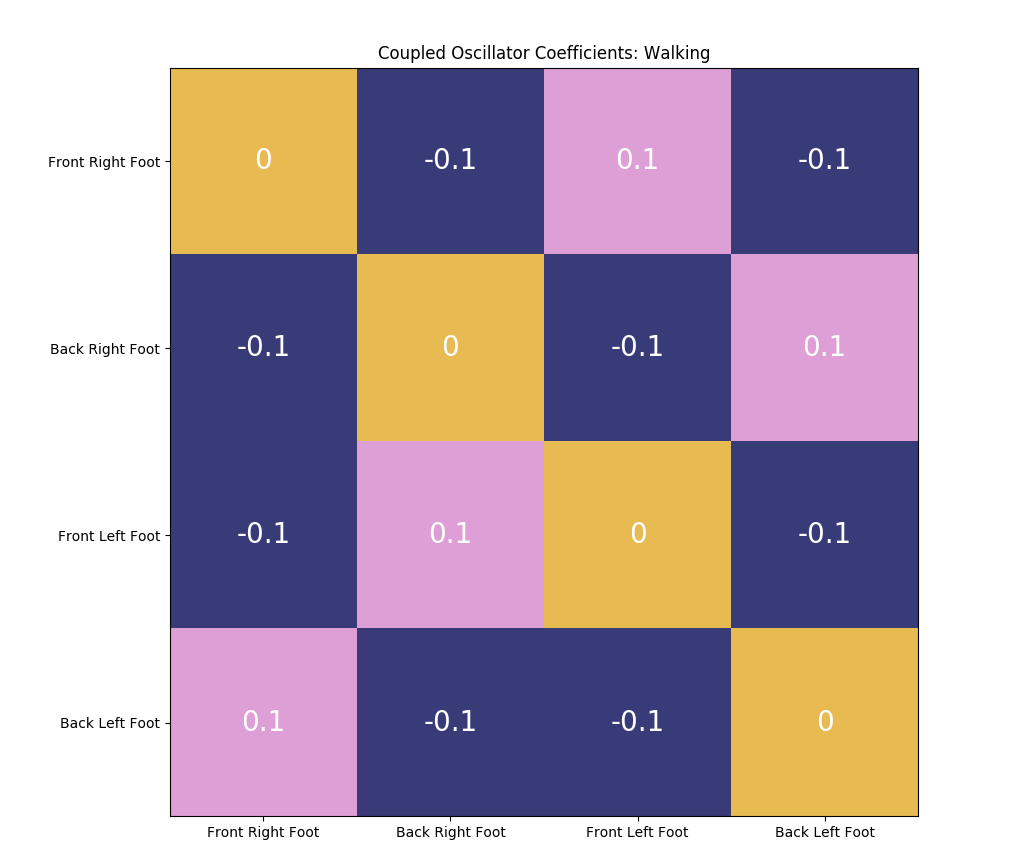
\includegraphics[width=0.33\textwidth]{USFD_Academic-_Report_LaTeX-Template/figures/walkingmatrix.png}
%         \caption{Walking Coupling Coefficients Matrix}
%         \label{fig:walk}
%     \end{subfigure}
    
%     \begin{subfigure}
%         \centering
%         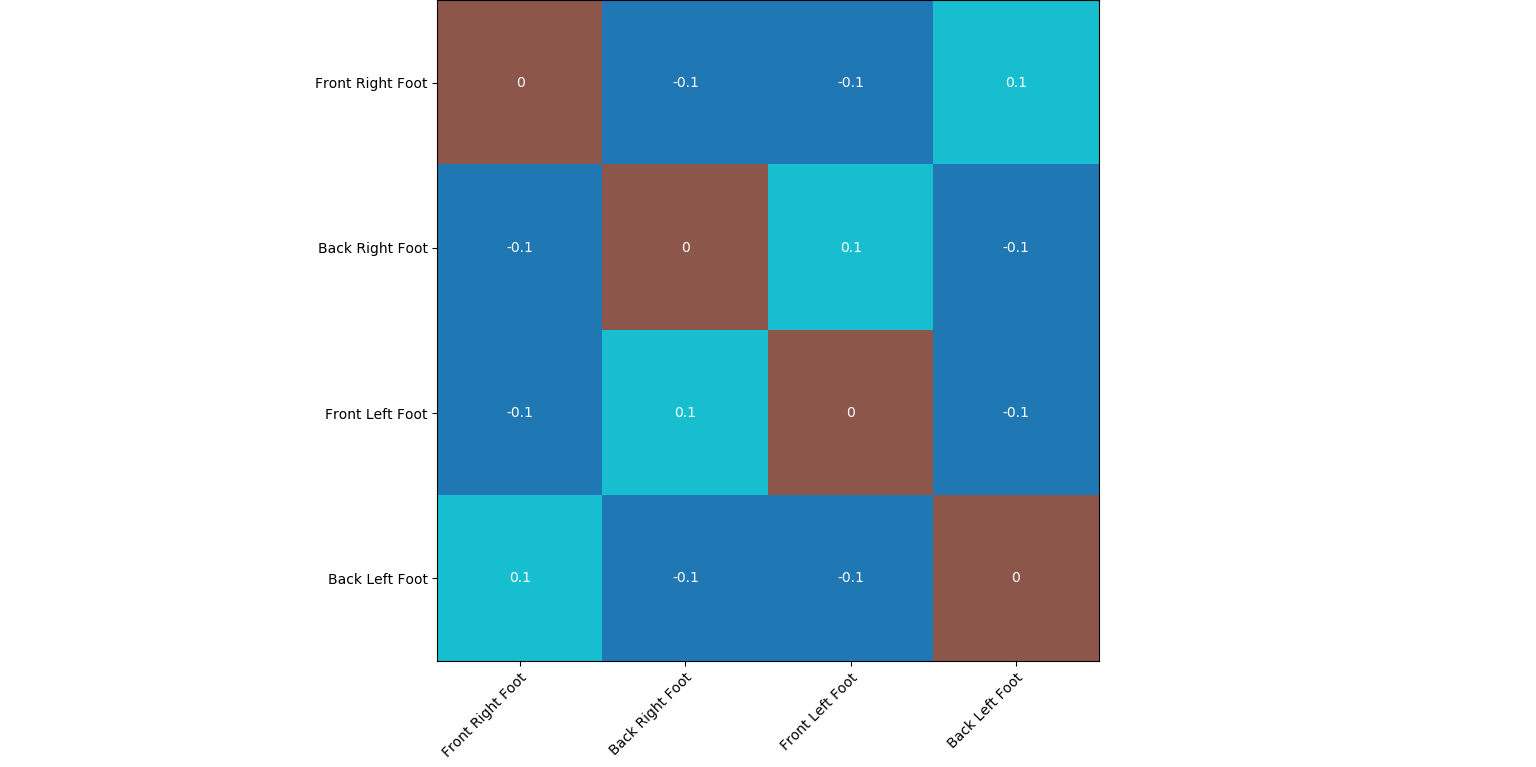
\includegraphics[width=0.33\textwidth]{USFD_Academic-_Report_LaTeX-Template/figures/trotosc.png}
%         \caption{Walking Coupling Coefficients Matrix}
%         \label{fig:walk}
%     \end{subfigure}
    
    % \begin{subfigure}
    %     \centering
    %     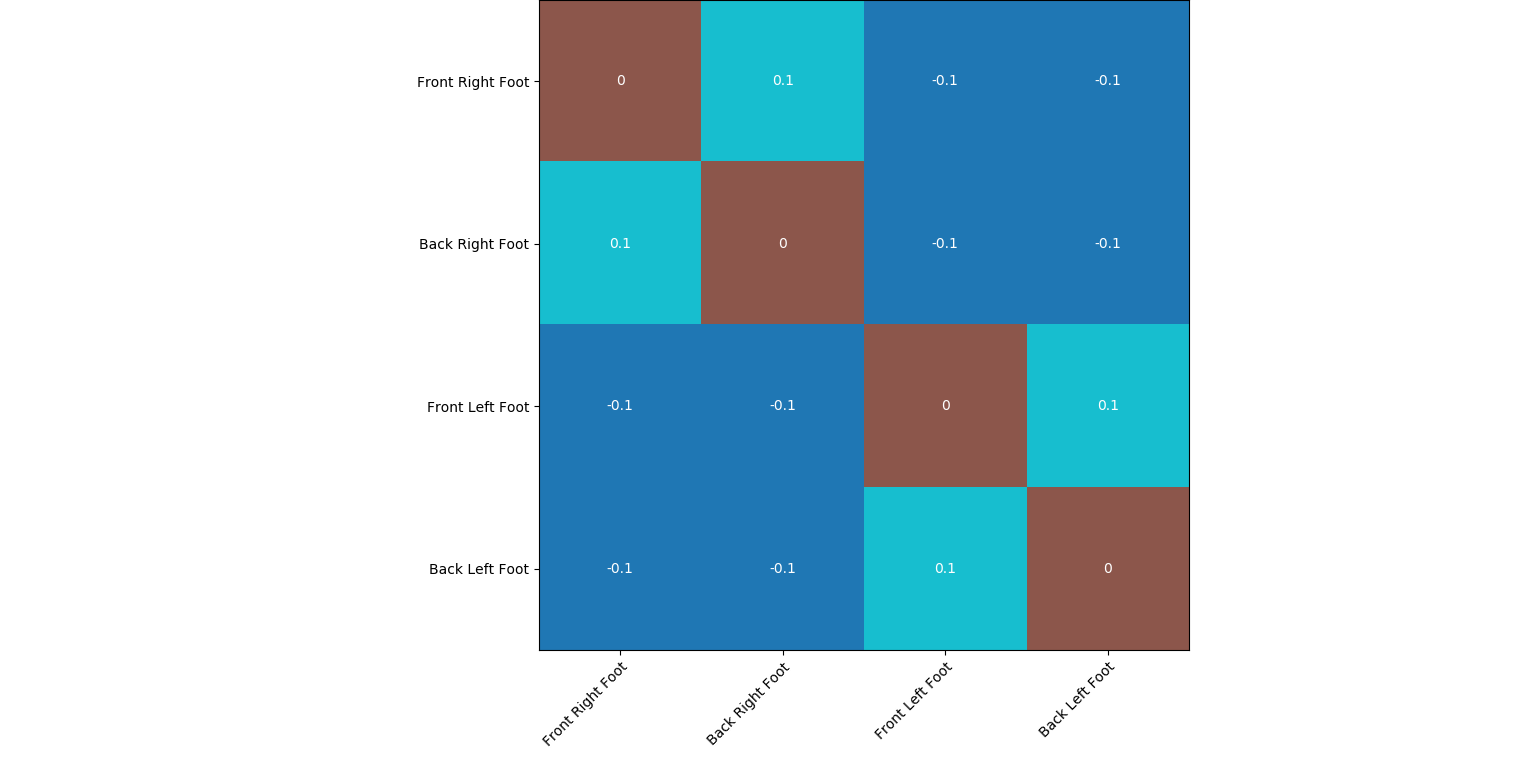
\includegraphics[width=0.33\textwidth]{USFD_Academic-_Report_LaTeX-Template/figures/osc_bound.png}
    %     \caption{Walking Coupling Coefficients Matrix}
    %     \label{fig:walk}
    % \end{subfigure}
% \end{figure}

After the implementation of the coupled Van der Pol generator to represent a CPG, the next stage of implementation is creating a robotic environment to investigate gaits.

\subsection{Robotic Environment}
This paper uses PyBullet for the creation of robotic simulation. PyBullet is a free open source physics engine which has shown success in simulating gait movement in this past. Recently, PyBullet was used in order to implement learned quadruped locomotion in \cite{Singla2018}. Additionally, investigation by \cite{Collins2018} has shown PyBullet to have extremely accurate conversion from a simulation to an actual robot, making the simulation the most appropriate for evaluating against real life values.

The robot used in this experimentation will be the Laikago robot, due it containing limbs in the Para-Saggital plane, making it a model of a Cursorial mammal. In addition using Deep Mimic, this has shown to recreate gaits successfully. 

The most appropriate form of simulation found is PyBullet's step simulation mode. PyBullet contains both step-simulation and real-time simulation. Real-time simulation replicates the processing over the current processor, while step simulation runs the next frame of simulation each time it is called. Step simulation was found to be the most appropriate as it will reduce the effects of computer processing in real time simulation on the robot. When investigated over using PyBullet's real-time option, the addition of extra monitoring changed the simulation time. This could cause issues with results testing as over time, the simulation may change due to extra processing strain on PyBullet.


% Each experiment has been repeated 10 times, and ran for 10000 iterations at time-steps of 1/500. 

Initially, before parameter testing, a successful gait was generated using the above Central Pattern Generator through values found in previous research, and trial and error. This was done in order to evaluate potential issues with the CPG design before experimentation. 

One of the issues seen with gait generation was rotation of the robot over time. This can be seen in \ref{fig:rotation}. This may be due to the lack of real time feedback of the robot, stopping the Laikago robot from correcting itself. An issue was found with the Laikago model, wherein the robot's centre of gravity was leaning to the side due to a mistake with motor masses. This issue was fixed, and the creator of PyBullet was contacted with the fixed version. Although this reduced rotation over time, it did not remedy the issue fully. As this would not be appropriate for a testing circumstance, due to the effects tilting may have on correctly finding distance travelled over time.

In order to investigate the difference between imaginary and actual oscillator values, the imaginary oscillator was transposed into the real oscillator, based on an inverse transposition at the end of 10000 iterations. An example of this transposition can be seen in \ref{}.  

\begin{figure}
    \centering
    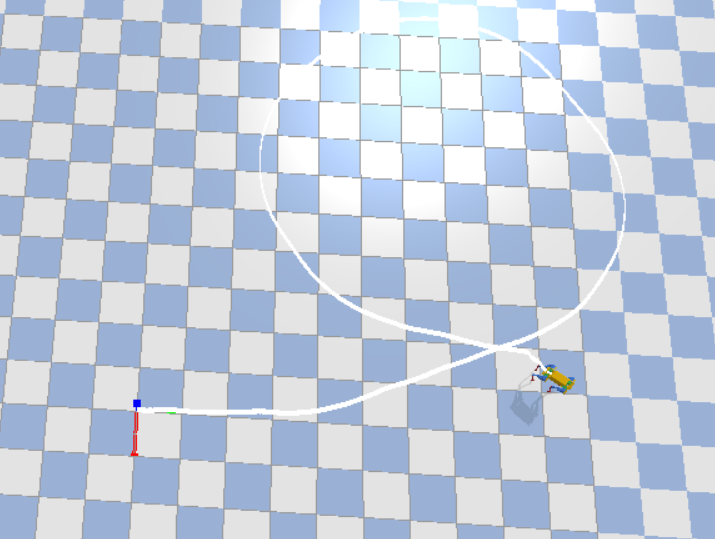
\includegraphics[width=0.65\textwidth]{USFD_Academic-_Report_LaTeX-Template/figures/rotation_over_time.png}
    \caption{Change in rotation over time. Path of robot indicated by white line}
    \label{fig:rotation}
\end{figure}

\section{Testing}
with a T test being ran between the two values, table \ref{} was found. The difference between the two values where found to be mostly negligible, and can be seen in \ref{fig:ttests}. Due to the extremely small P-values found in the T-tests, it shows that there is not a large effect on virtual oscillator values being moved into simulated limbs. This change may be far larger for implementation into an actual robot, and as such, may cause issues with gait generation, however, the extremely low p-values found suggests that there is potential in accurate conversion for actual robots. 

In order to create a suitable testing environment, two walls where created on either sides of the robot in order to reduce measurement complexity and reduce the effect of balancing issues may have on the robot, as issues with the robot collapsing in the middle of its gait may cause inaccurate measurements of Froude number. This reduces the effects seen by the robot tilting over time.

A similar method of parameter search as found in \cite{Rutishauser2008} was decided due to needing a wide range of different Froude number values when comparing against the Dynamic Similarity Hypothesis. This was through the use of evaluating against a large combination of parameters and building a matrix table of successful results. Initially, we investigated two main parameters, max-force and speed of oscillations against a full set of gaits. 

As can be seen from \ref{}, this found that the minimum force value for all gaits 15N. Below this, the robot could not sustain it's own weight. Above 120N all gaits, however, both trotting and walking experienced cut offs at both 80N.

A slight change has been  made to the amount of iterations after implementation, due to coupling causing an effect where the oscillators take more time than expected to get into positions. This can be seen through \cite{}. Due to this effect, the iteration size has been increased to 11000, with the first 1000 iterations being ignored in calculations, to both allow the PyBullet engine to process the initial placement of the robot (which caused errors in force calculations, as can be seen from \cite{}).


% Walking, trotting and bounding where initially investigated over various force values, each experiment was repeated 10 times, for a total of 11000 iterations at timesteps of 1/500s, with the experiments being ran in PyBullet step simulation to reduce potential issues with processing. 

% In order to investigate the amount of values that are kept within the confines stated by \cite{Alexander1983}, The experiments where for values across the valid ranges described. This was done in order to get a wide range of values that are kept within the confines seen to produce successful gaits. 

% One of the issues faced in this dissertation was reducing the difference between imaginary oscillator gaits and actual force output on limbs. Due to the robot moving forwards, especially at lower force levels, the output of van-der-pol oscillators did not translate exactly to the real motor values. This can be seen through the graph below, which used force values of (), oscillator values of (), along with a leg rotation of (), and a hip rotation of ().
% Although this shows a clear increase towards similarity as force increases, this does not translate directly to ideal gait performance. 



% have decided to adapt the oscillator parameters seen in \cite{} for initial experiments, making the oscillator take the following form, which is described in \cite{}.


%   % Replace with your text
% \begin{equation}
% \ddot{x} + \alpha(x^2 - 1)\dot{x} + x = 0
% \label{vanderpol:pure}
% \end{equation}

% \begin{figure}
%     \centering
%     \includegraphics[width=1\textwidth]{figures/oscillatoroutput.png}
%     \caption{Dynamics of Van Der Pol Oscillator}
%     \label{fig:vanderpolpure}
% \end{figure}

%  This can be simplified through the use of the transformation ${\dot{x} = y}$, which allows our oscillator to take the form found in \ref{vanderpol:twod}


\chapter{Results \& Discussion}
\section{Results}


Through investigating the walking gait on a large proportion of values, the following data was gathered. A full table of experiments ran can be found in the appendix. 

Figure \ref{froudedistribution} showcases the probability distribution of all values found. The probability distribution showcases a mean  with a Froude number of 0.358, with a variation of 0.283. This is a fairly large variation, which may be due to a large amount of values finding themselves at very low gait values. This show a close adherence to Dynamic Similarity, with a bulk of values finding themselves below gaits of 0.4. In total, out of all of the experiments ran, 72.4\% of values where found to lie below 0.4. 

\begin{figure}[h!]
  \centering
  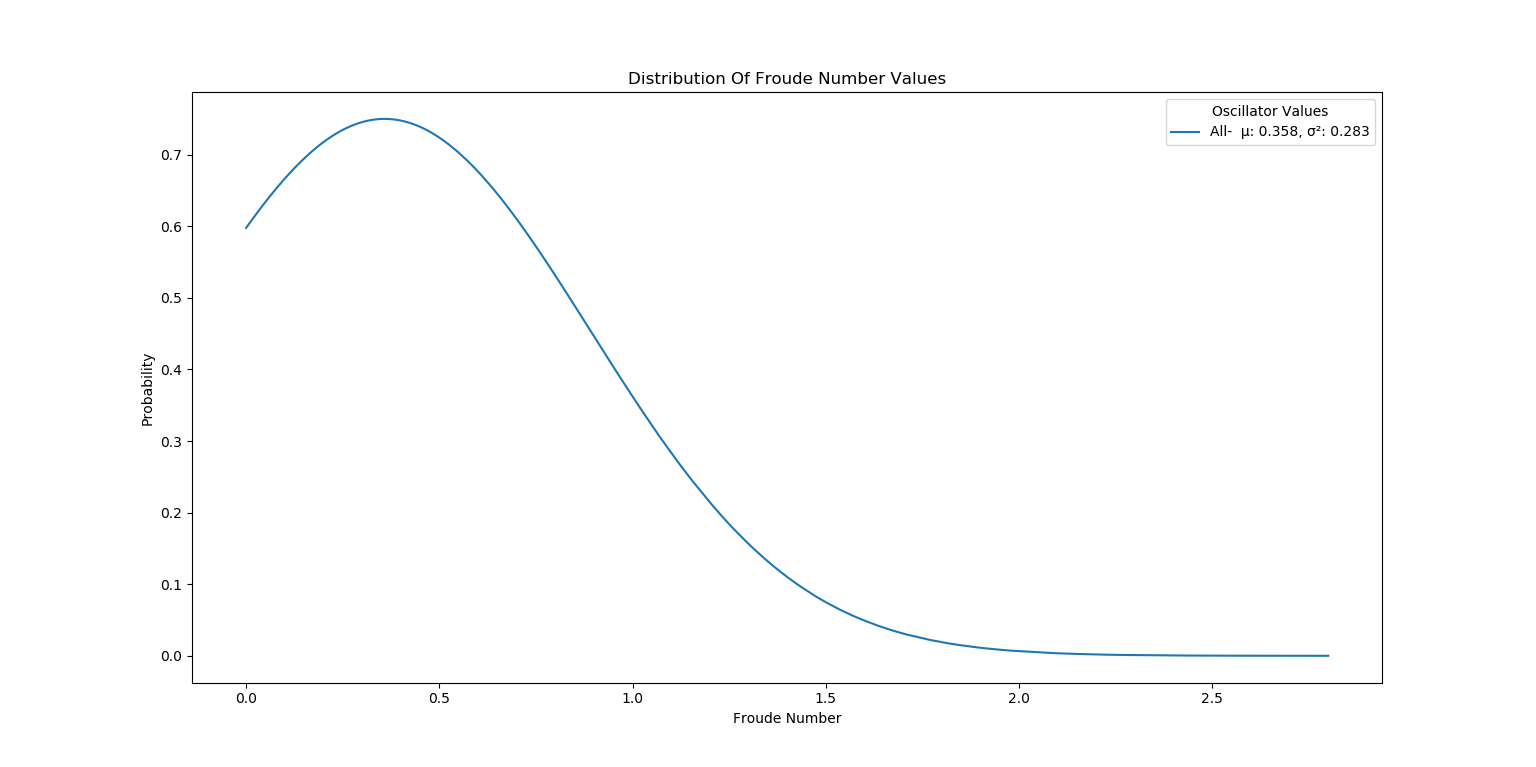
\includegraphics[width=1\textwidth]{USFD_Academic-_Report_LaTeX-Template/figures/froudedistribution.png}
  \caption{Distribution of froude number for all experiments.}
  \label{froudedistribution}
\end{figure}

This distribution does showcase that a large proportion of values are still above 0.4. This does not correlate with the Dynamic Similarity principle, in which Froude numbers of 0.4 are described as the maximum for an animals walking gait, with walking gaits above 0.4 not being seen. An explanation as to why this appears to be due to oscillator time-step, as when filtering the results against oscillator time-step, the distribution seen in figure \ref{froudeosc} are achieved.

\begin{figure}[h!]
    \centering
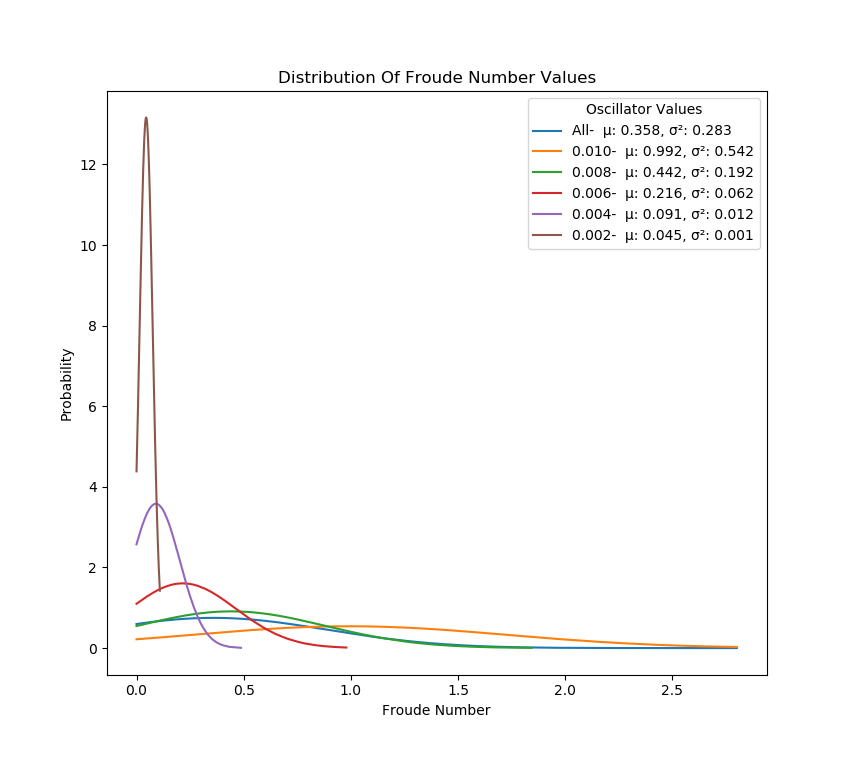
\includegraphics[width=1\textwidth]{USFD_Academic-_Report_LaTeX-Template/figures/froudedistributionoscillator.png}
\caption{Distribution of froude number by oscillation.}
\label{froudedosc}
\end{figure}

This shows that the majority of larger values are found due to larger oscillator time-steps. Above values of 0.008, the mean increases to values far above the range seen in \cite{Alexander1983}. When filtering by oscillator time-steps of 0.006 and below, find that () of results lie within the limits found in Dynamic Similarity. 



% The effects on Froude number when varying forces are far less pronounced, as can be seen through \ref{}
% \begin{figure}[h!]
%     \centering
% \includegraphics[width=1\textwidth]{USFD_Academic-_Report_LaTeX-Template/figures/froudevsforce.png}
% \caption{Distribution of froude number by oscillation.}
% \label{froudefocre}
% \end{figure}

% Although the values reach a peak between 60 and 70, after these values the Froude number reduces. This may be due to a higher variation between values at this point, which suggests that after this point, a large amount of the gaits produced may be unstable

% \section{Cost Of Locomotion}
% Cost of locomotion has been calculated using research shown by \cite{}. Cost of locomotion has been calculated by the following equation.

% Due to the experiment running for a set amoiunt of iterations instead of distance, for this paper, we will be using the cost of locomotion per unit distance travelled. This is in order to allow comparisons between cost of locomotion and velocity, as a robot travelling at a larger velocity may be less efficient than one travelling slower.

% \begin{figure}[h!]
%   \centering
%   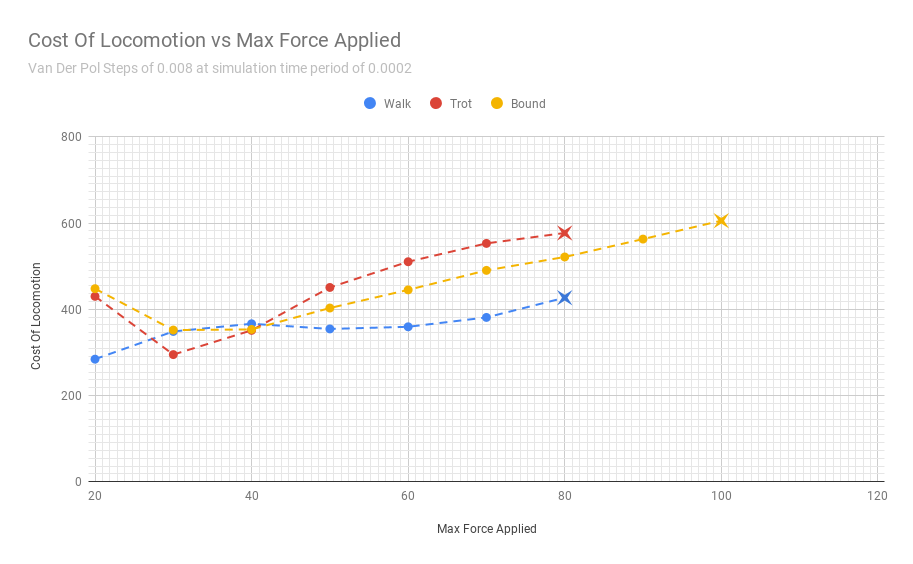
\includegraphics[width=1\textwidth]{figures/fig2.png}
%   \caption{Cost of locomotion per unit distance over force applied.}
%   \label{walktrotbound}
% \end{figure}

% \begin{figure}[h!]
%   \centering
%   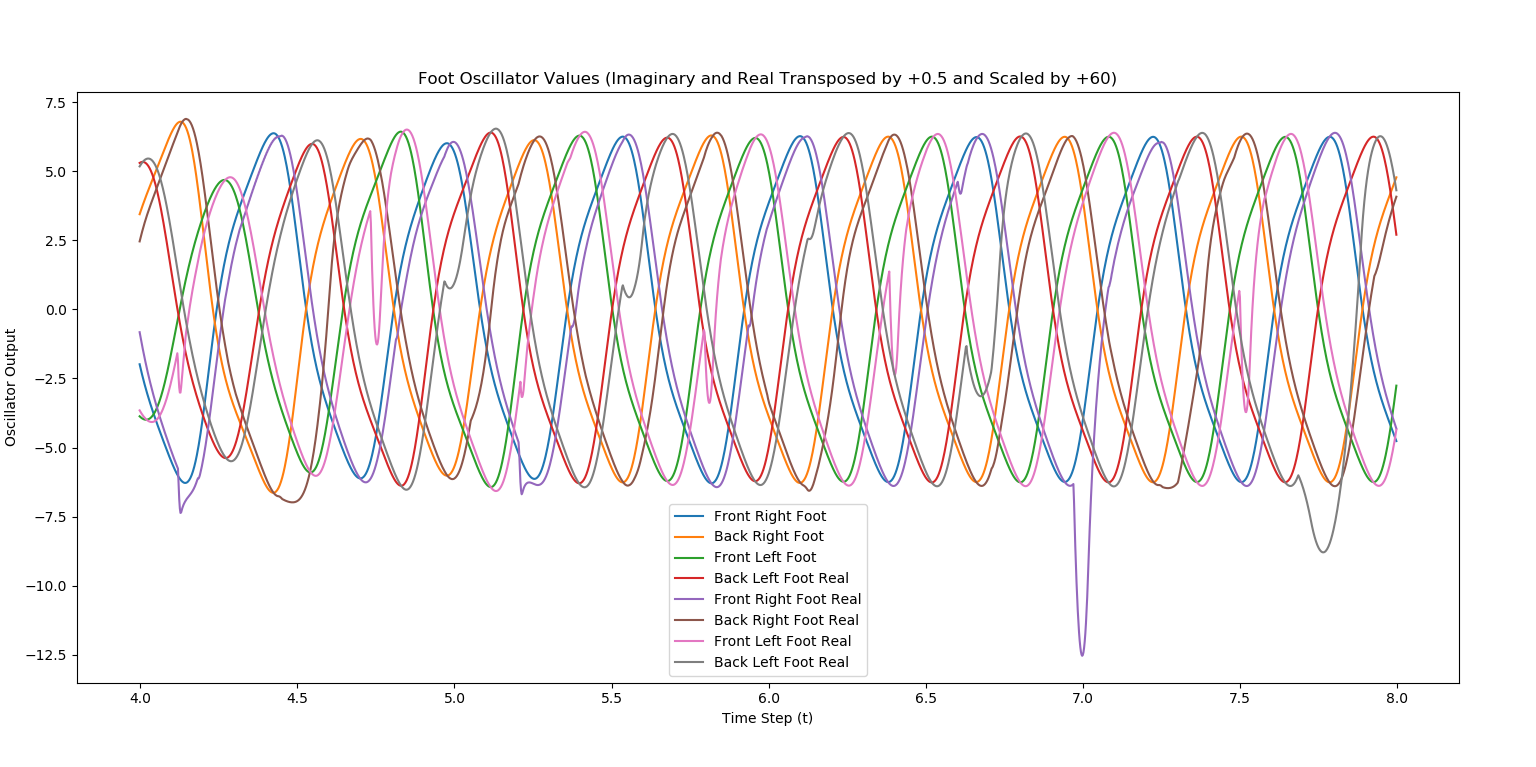
\includegraphics[width=1\textwidth]{USFD_Academic-_Report_LaTeX-Template/figures/oscillatortranspose.png}
%   \caption{Results of reverse transposition and scaling real motor outputs onto oscillator values.}
%   \label{walktrotbound}
% \end{figure}


% \begin{figure}[h!]
%     \centering
%     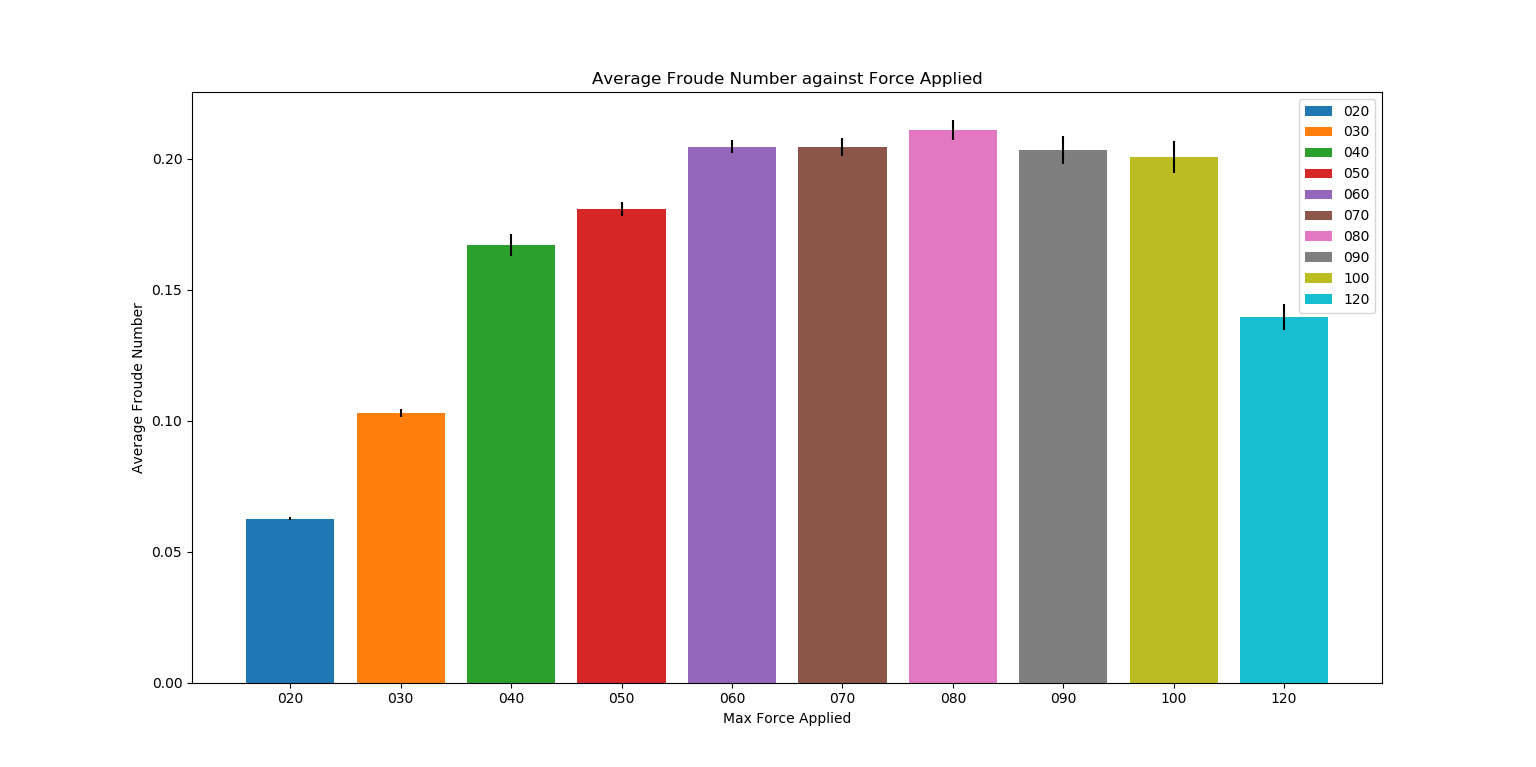
\includegraphics[width=1\textwidth]{USFD_Academic-_Report_LaTeX-Template/figures/froude_number_against_force.png}
%     \label{froudenumbervsforce}
% \end{figure}

% \begin{figure}[h!]
%     \centering
%     \includegraphics[width=1\textwidth]{figures/froudevsforce.png}
%     \caption{Average Froude number against force applied for entire dataset of experiments.}
%     \label{froudenumbervsforce}
% \end{figure}


% \begin{figure}[h!]
%     \centering
%     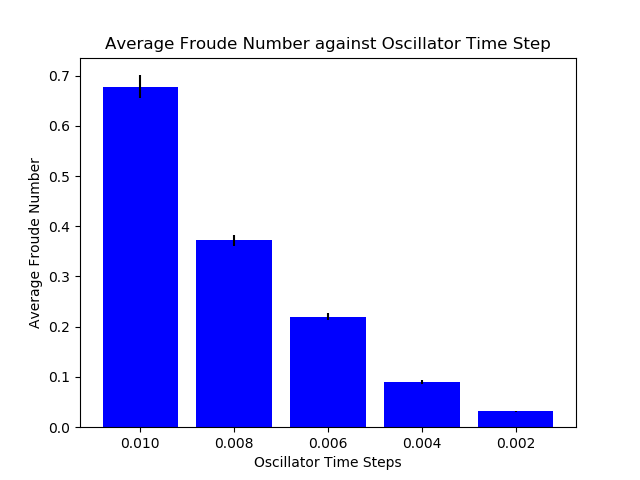
\includegraphics[width=1\textwidth]{figures/froudeosc.png}
%     \caption{Average Froude number against change in oscillator time-step for entire dataset of experiments.}
%     \label{froudenumbervsoscill}
% \end{figure}

% \begin{figure}[h!]
%     \centering
%     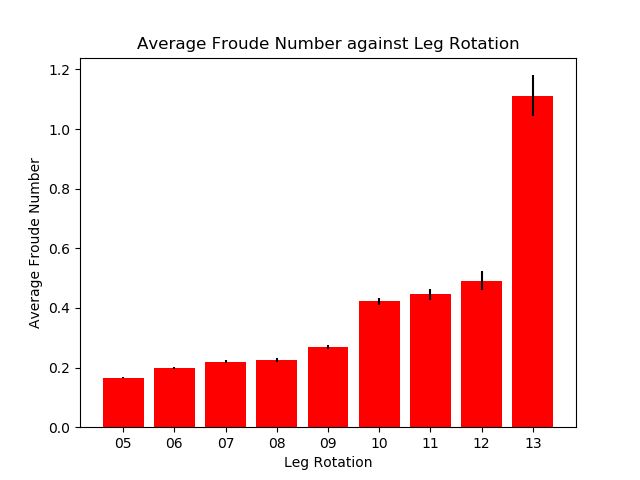
\includegraphics[width=1\textwidth]{figures/froudevsrotation.png}
%     \label{froudenumbervsangle}
%     \caption{Average Froude number against leg rotation for entire dataset of experiments.}
% \end{figure}



% \section{Dynamic Similarity}
% For this paper we will investigate specifically the results seen in relative stride length against froude number, as they are the closest calculation available to be performed. Froude number was investigated against changes in parameter. We focused on the  walking gait in this dissertation due to the large complexity of the system, and the results seen in the initial gait analysis, as even in higher forces, faster gaits still broke down at similar values. This in return can be displayed through a normal graph, as can be seen in 

% \begin{figure}[h!]
%     \centering
%     \includegraphics[width=1\textwidth]{figures/forceandnormal.png}
%     \label{froudenumbervsangle}
% \end{figure}


% Some investigation was done into force values below 20, but we found that this ended with the robot being unable to keep it's own weight. The results of that investigation can be seen in the table in the appendix. 

\section{Discussion}
One of the most interesting results is through the investigation of Froude number values when applying a walking gait. The majority of results for walking gaits, irregardless of oscillator time step, foot angles, or force applied have remained in the regions seen in \cite{Alexander1983}. Namely, Froude numbers below 0.4. As stated in the results, this does mean that almost 30\% of values reach above the limits imposed, however when filtering by oscillator time step, There was an increase the amount of values found in the correct range by (). This shows that the majority of values found above Froude numbers of 0.4 where due to higher oscillator time-steps. These oscillator time-steps may not be attainable realistically as this dissertation did not take into account factors of interlimb friction that may occur in an actual robot/ quadruped mammal. Because of this, it may be that there is a physical limit that does not exist with our robot at faster oscillations. This additionally would suggest that the limiting factor in velocity of a walking gait is the speed the limbs can move at. 

% This can be seen through the following graph. Although there appears to be a steady increase as both oscillator values and rotation angles are increased, this is additionally marked by a high change in variance, making gaits far less stable to changes in force at these values. 



Additionally, maximum gait values in this design are only reaching upwards of 2.0, meaning they remain in the lower bounds of faster gaits. This may be a reason as to why effects of faster gaits have not been successful in this research. This may be due to potential issues with the implementation of our model. This is extremely similar to the results found in \cite{Rutishauser2008}, although the implementation of a Central Pattern Generator is different. This suggests that the implementation of faster gaits such at trots may require additional balancing through the use of real-time feedback. 

Another potential issue which may have skewed the results, and caused faster gaits to be unsuccessful could potentially be caused due to the Laikago model used in the dissertation not having completely accurate mass values. As stated in the implementation stage, although 

% One of the potential reasons as to why many values where found outside of the appropriate bounds of walking may be due to the motors not taking into account real friction that would be seen in animal limbs, although linear damping was set, it may not be fully realistic. The motors themselves where controlled by the velocity control option in PyBullet. 

% As stated in \cite{Alexander1983}, the majority of animals display walking gaits below 0.4. For all of the results in this dissertation, irregardless of force, oscillator time-step or limb rotation, we found that \% of values achieved adhered to this value of froude number.

% Overall, 60.2\% of values where under froude numbers of 0.4, which links towards the same values being found for the majority of animal gaits as seen in \cite{Alexander1983}. The amount of values found above this may be due to the lack of friction against limbs in the environment. This effect is most pronounced on oscillator time-steps of (), where 78\% of values where found to lie under.



% The effects of leg rotation on froude number showcase that there may be a large effects on froude number depending on leg rotation. However, similarly to changes in force, larger changes in leg rotation are met with larger deviations, with stable gaits occuring below a froude number of 0.4. 

% A covariance matrix between cost of locomotion and froude number can be seen below, showcasing how changes in cost of locomotion affect froude number. 

% This seems to coincide with froude number research, and suggests that although our simulated robots can use far faster gaits, there is a higher effect on variation, and as such, walking gaits that use larger angle values may perform faster gaits outside of the range seen in evolutionary circumstances. Although these may be out of range they are essentially symmetric gaits. The reasons as to why a walking gait may still perform well outside of this range is that the 

% Due to the normal distributions seen by the data, as can be seen through






% Distribution was calculated for all experiments ran, with distribution gathered for froude number and cost of locomotion. Froude number distribution can be seen in \ref{froudedistribution} and cost of locomotion distribution can be seen in \ref{costdistribution}. They will be discussed together due to both of them having extremely high continuous distributions with positive skew. Particularly, they both show that there is an extremely large amount of results at, or close to 0 for both froude number and cost of locomotion. This suggests that many of the gaits prove to be unstable and do showcase realistic gait values. Although froude number is shown to be very low in \cite{Alexander1983}, this is still worrying. The following can be seen by filtering the distributions based on force. This showcases the effect that force has on gait value, with variance increasing as force increases. 





% \begin{figure}[h!]
%   \centering
%   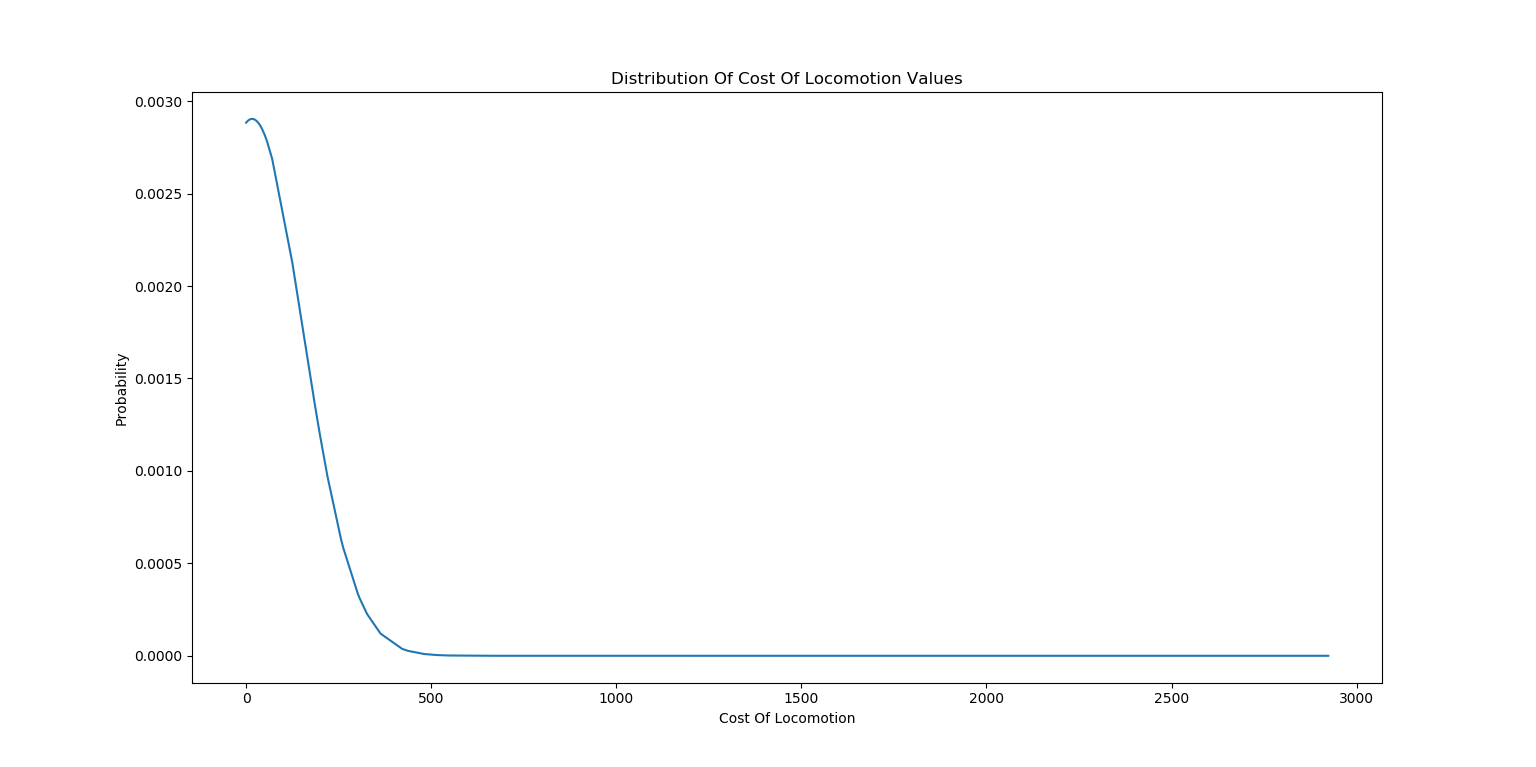
\includegraphics[width=1\textwidth]{USFD_Academic-_Report_LaTeX-Template/figures/costoflocomotiondistribution.png}
%   \caption{Distribution of cost of locomotion per unit distance.}
%   \label{costdistribution}
% \end{figure}

% \begin{figure}[h!]
%   \centering
%   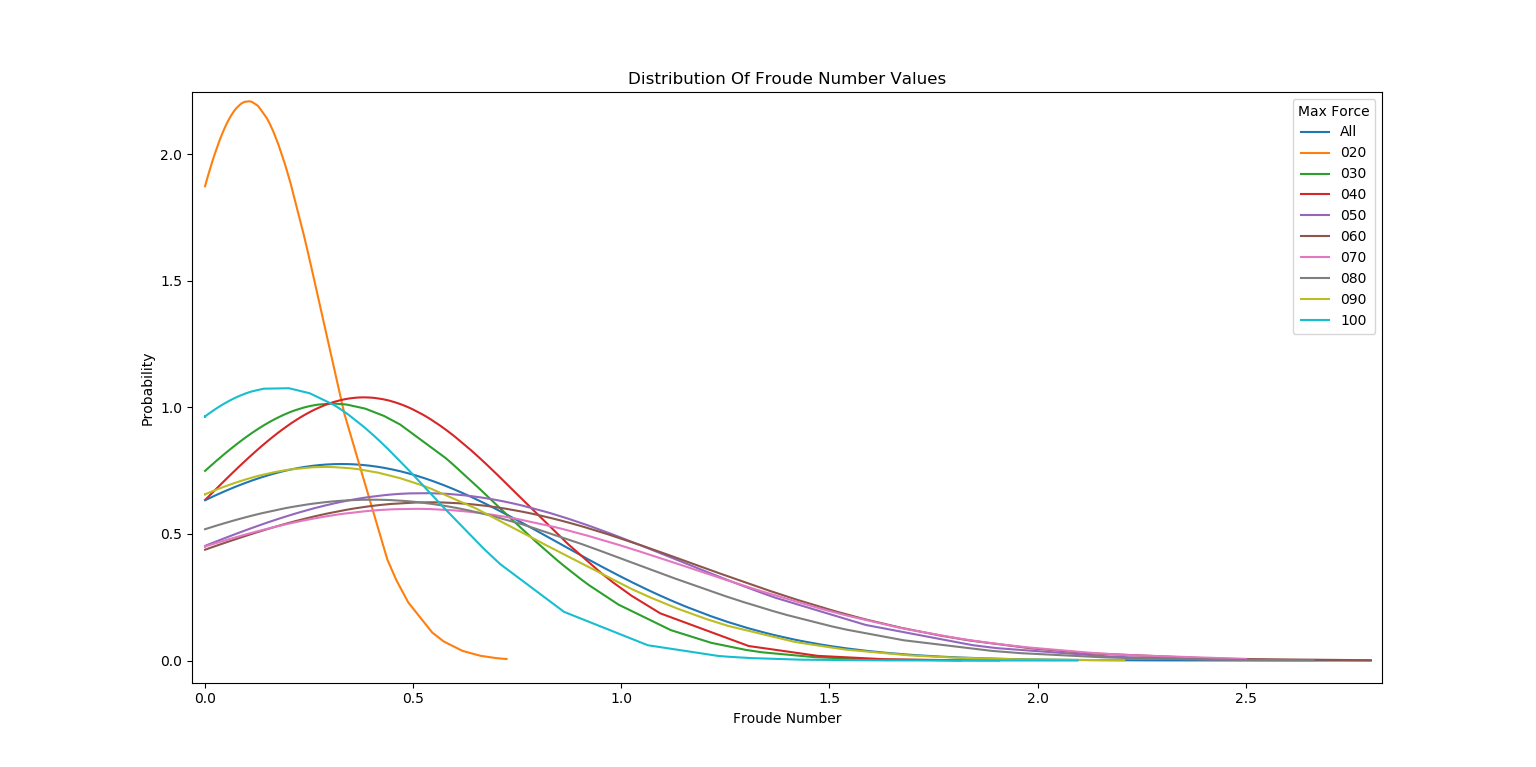
\includegraphics[width=1\textwidth]{USFD_Academic-_Report_LaTeX-Template/figures/froudenforcedistributions.png}
%   \caption{Distribution of cost of locomotion per unit distance.}
%   \label{costdistribution}
% \end{figure}

\section{Further Work}
 Due to the accuracy of pybullet when converting from simulation to real robotics, as seen in \cite{}, further research could be done on comparing the results seen in this work to an actual quadruped robot. As the models seen in this work have been directly based on the Laikago robot, a direct comparison could be made between the experimental results found and actual gait results generated. If a full system identification of the Laikago is made, this could increase the accuracy of the results seen in the paper.

This paper has only dealt with gaits in a limited environment with the test environment confining the animal to travel down a straight line. With the implementation of limb feedback, additional work could be done in effects on the animals CPG through the introduction of obstacles in the environment. More work could potentially be done on the introduction of control into the system, allowing the gaits to change dynamically based on the velocity chosen, as well as a possible implementation of turning through changing coupling.

An interesting, although slightly peculiar potential method for future work is an investigation as to whether the dynamic similarity hypothesis will still hold for different gravity values, as it is part of the equation for Froude Number. This would be an interesting method as it could potentially highlight speeds and gaits that animals should be travelling at in different bodies. For example, if a quadruped robot is attempting to travel on the moon, it would in turn not need to use anything faster than a walking gait, as it would be able to achieve the same velocities without expending as much energy.  

Although out of scope for the project due to time constraints, further work can be done on implementing evolutionary techniques for this project, due to the large amount of free parameters found in this system. This could be done with a similar method as seen in \cite{Geijtenbeek2013}. This could however cause issues with comparisons between Dynamic Similarity, due to faster gaits being possible. A possible solution to this would be investigating different cost functions for robot, such as stability or velocity and comparing them to a cost function related to adhering to Dynamic Similarity. This could show reasons as to why mammals might adhere to the concept of Dynamic Similarity, and provide a new cost function that can be used when designing quadruped mammals.

 Additional work should be done investigating the effectiveness of faster gaits at larger values. One of the main issues with using faster gaits for this project was due to stability, as the robot did not contain any methods of remaining stable when using faster gaits, causing it to fall down when attempting to go quickly. By the implementation of feedback for walking, as well as potential balancing methods as seen in \cite{}, faster gaits, as well as transitions between gaits could be investigated.

After querying the creator of the pybullet engine, it was found that a full system identification had not yet been performed, and as such a 3D model with fully realistic values was not yet implemented in the engine. Once this system identification is complete, there is a potential in re-doing the experiments found in this dissertation, as the full system identification could include more in depth methods such as motor friction.

% Additional work could potentially be done on the application of dynamic similarity to different quadrupeds, through the extension of work done on different models, as the central pattern generator designed in this paper could easily be extended to different robotic models.





% \chapter{Discussion}

\chapter{Conclusions}
% A plan of the work can be seen in \ref{fig:gantt}. The main bulk of the work after the literature review will be the creation of a quadruped robot, however, we have left a large amount of time into graph and data creation, and correct experiment development, as more work needs to go into developing a scientifically valid experiment for do gait generation. Although my plan does not currently contain a time allowance for getting a physical robot, we believe it would replace the time taken to implement other machine learning methods, as it is not an integral part of this dissertation.

% \begin{figure}[ht]
% 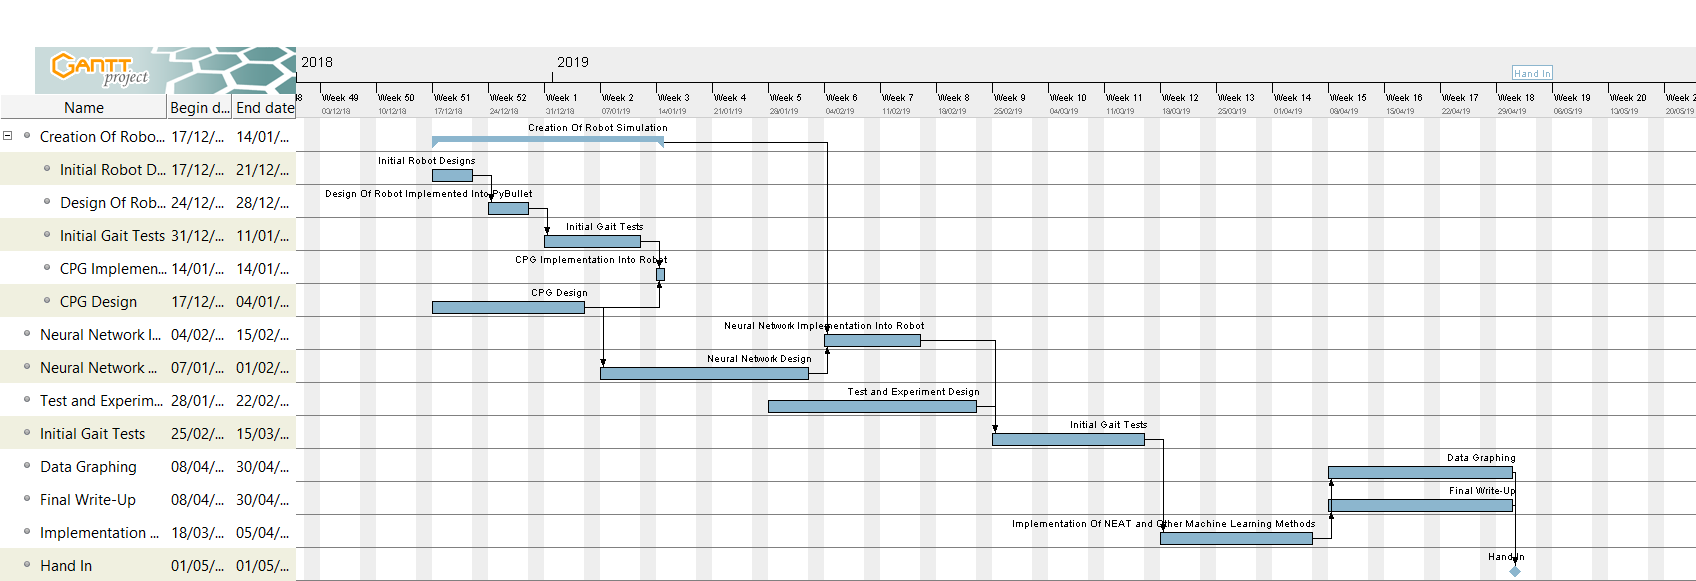
\includegraphics[width=15cm]{figures/gantt.png}
% \caption{A gantt chart showing the current project plan (www.ganttproject.biz)}
% \label{fig:gantt}
% \end{figure}

The work done in this paper provides a starting point for the creation of realistic animal gaits and additionally provides a platform through which other research may be done. As currently there does not exist an open source method of simulating and measuring animal gaits on quadrupeds, this research could provide a potential starting point for the development of realistic animal movements.

One of the main findings of this paper, was that irregardless of parameters tested, over 70\% of walking gaits performed tended within the amounts seen in the research of \cite{Alexander1983}. This shows that although it may be possible to 'cheat' evolutionary concepts and reach higher values than seen in evolutionary principles, to do so requires extremely fast repetition of gaits, which may be feasible in a step-simulation based environment, but might not apply to a real robot. 

This paper shows a valid initial breakdown of the effects of changing different parameter values on a simulated robot, with a valid comparison to Froude numbers found in mammals. This work additionally provides a basis for the measurement and creation of animal gaits, building a solid foundation from which other investigations can occur. 

Although this paper builds a foundation for the generation of simple gaits, only finds effective gait reproduction with walking gaits. This may be due to faster gaits requiring additional real-time feedback or methods of dynamic balancing. Similar issues have been found as in \cite{Rutishauser2008}, wherein a trotting gait does not produce gaits faster than walking. Although this research shows promising results for walking gaits, a more in depth study needs to be made for other gaits.


% -------------------------------------------------------------------
% Bibliography
% -------------------------------------------------------------------

\bibliographystyle{agsm} 
\bibliography{mybibliography} 


% -------------------------------------------------------------------
% Appendices
% -------------------------------------------------------------------

\begin{appendices}
 \chapter{Appendix A: Tables}


\chapter{Appendix B: Additional Figures}

% \begin{figure}
%     \centering
%     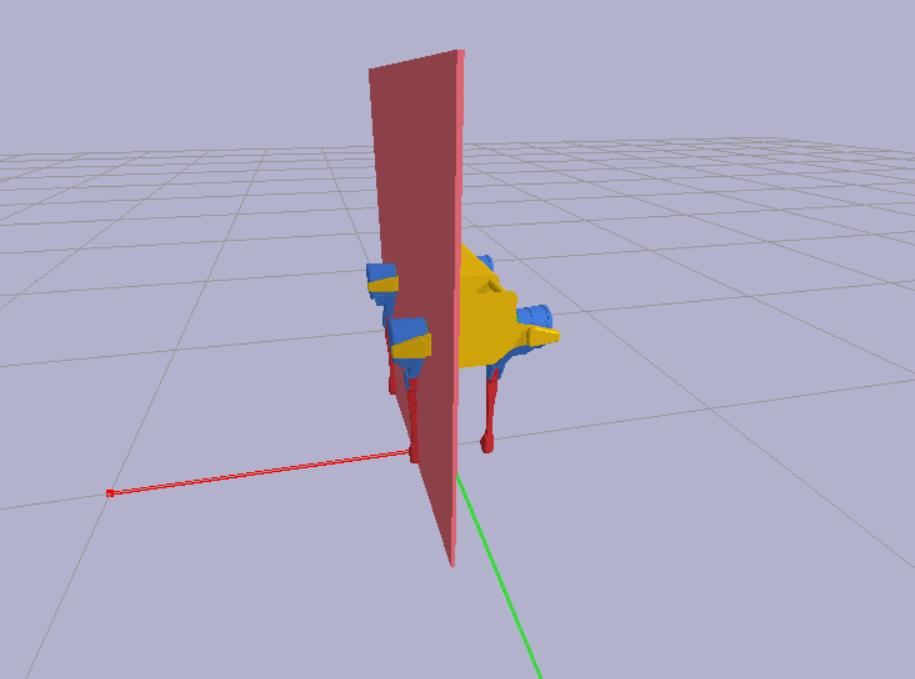
\includegraphics[width=1\textwidth]{figures/parasaggital.png}
%     \caption{Diagram of robot planes, the red square indicates the robots Parasaggital plane.}
%     \label{fig:parasaggital}
% \end{figure}
% \begin{figure}
%     \centering
%     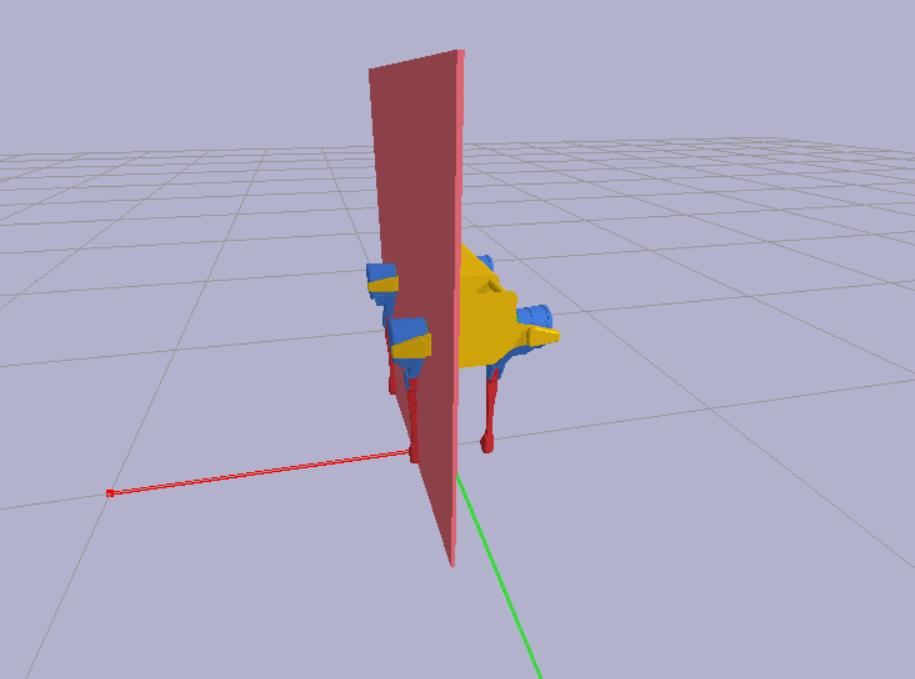
\includegraphics[width=1\textwidth]{figures/parasaggital.png}
%     \caption{Diagram of robot planes, the red square indicates the robots Parasaggital plane.}
%     \label{fig:parasaggital}
% \end{figure}
% \begin{figure}
%     \centering
%     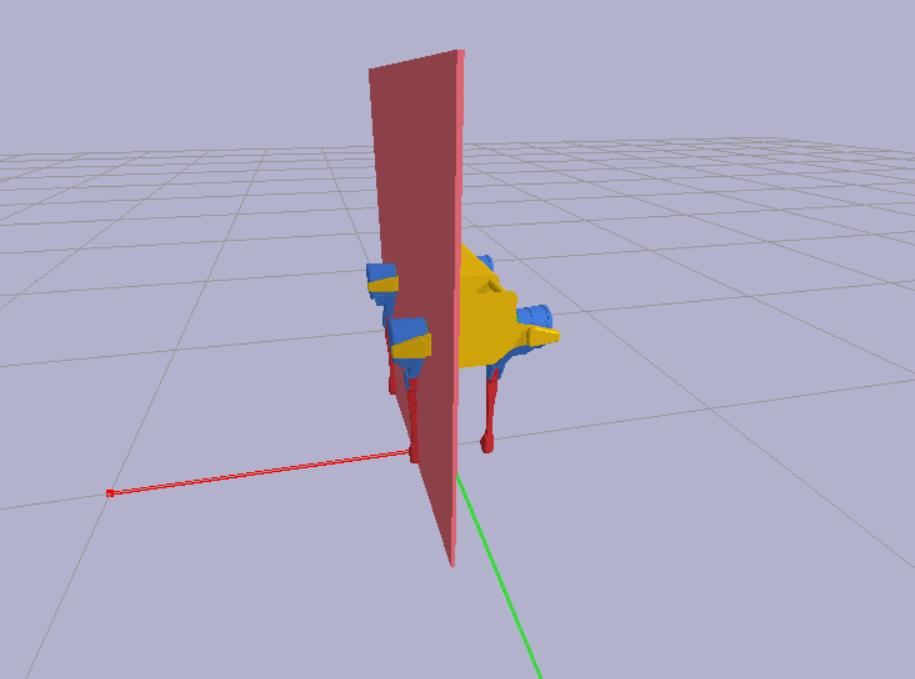
\includegraphics[width=1\textwidth]{figures/parasaggital.png}
%     \caption{Diagram of robot planes, the red square indicates the robots Parasaggital plane.}
%     \label{fig:parasaggital}
% \end{figure}

\begin{figure}[h!]
    \centering
    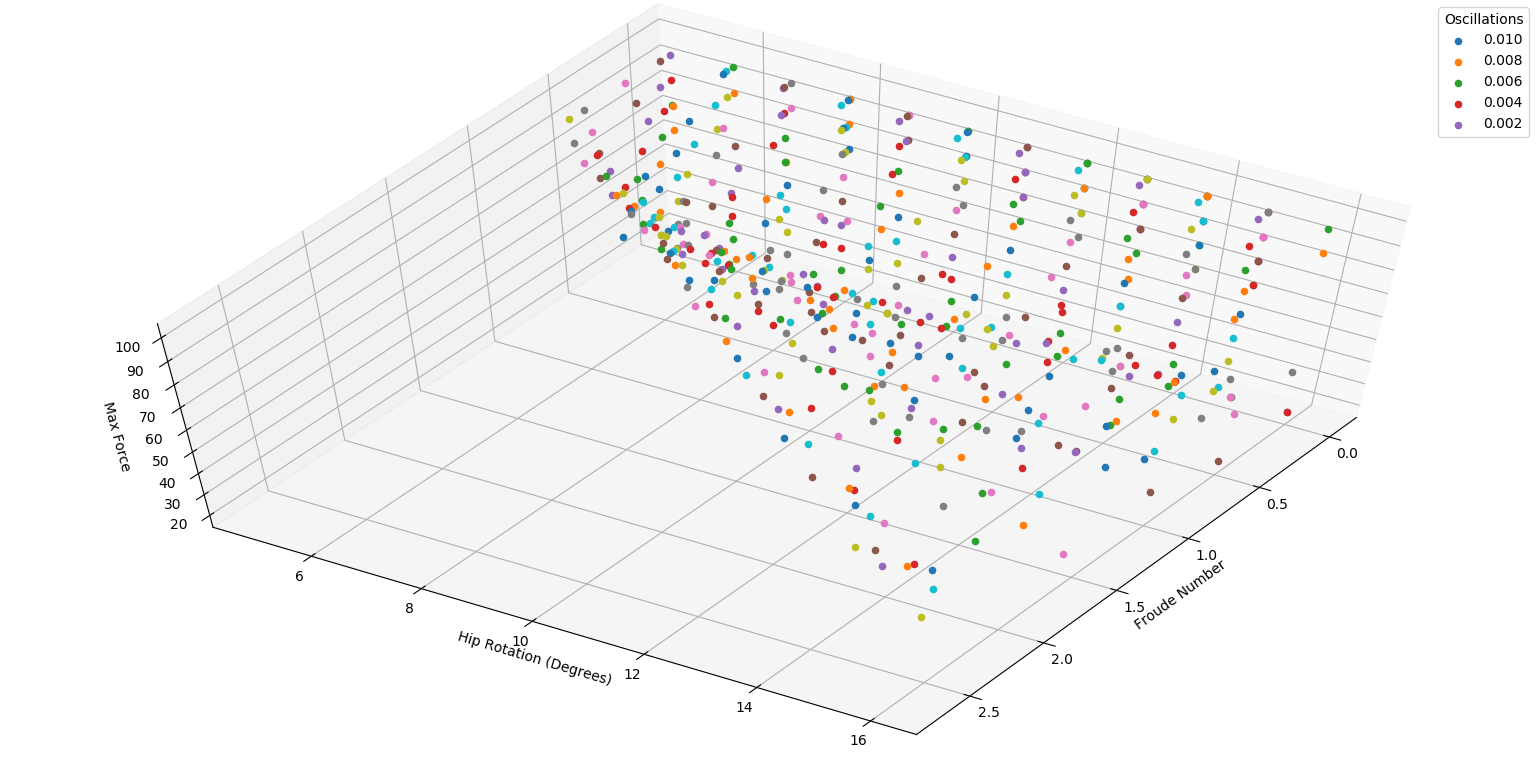
\includegraphics[width=1\textwidth]{figures/forcerotationfroude1.png}
    \label{froudenumbervsangle}
    \caption{All variation of experiments shown on 3D graph, view 1}
\end{figure}

\begin{figure}[h!]
    \centering
    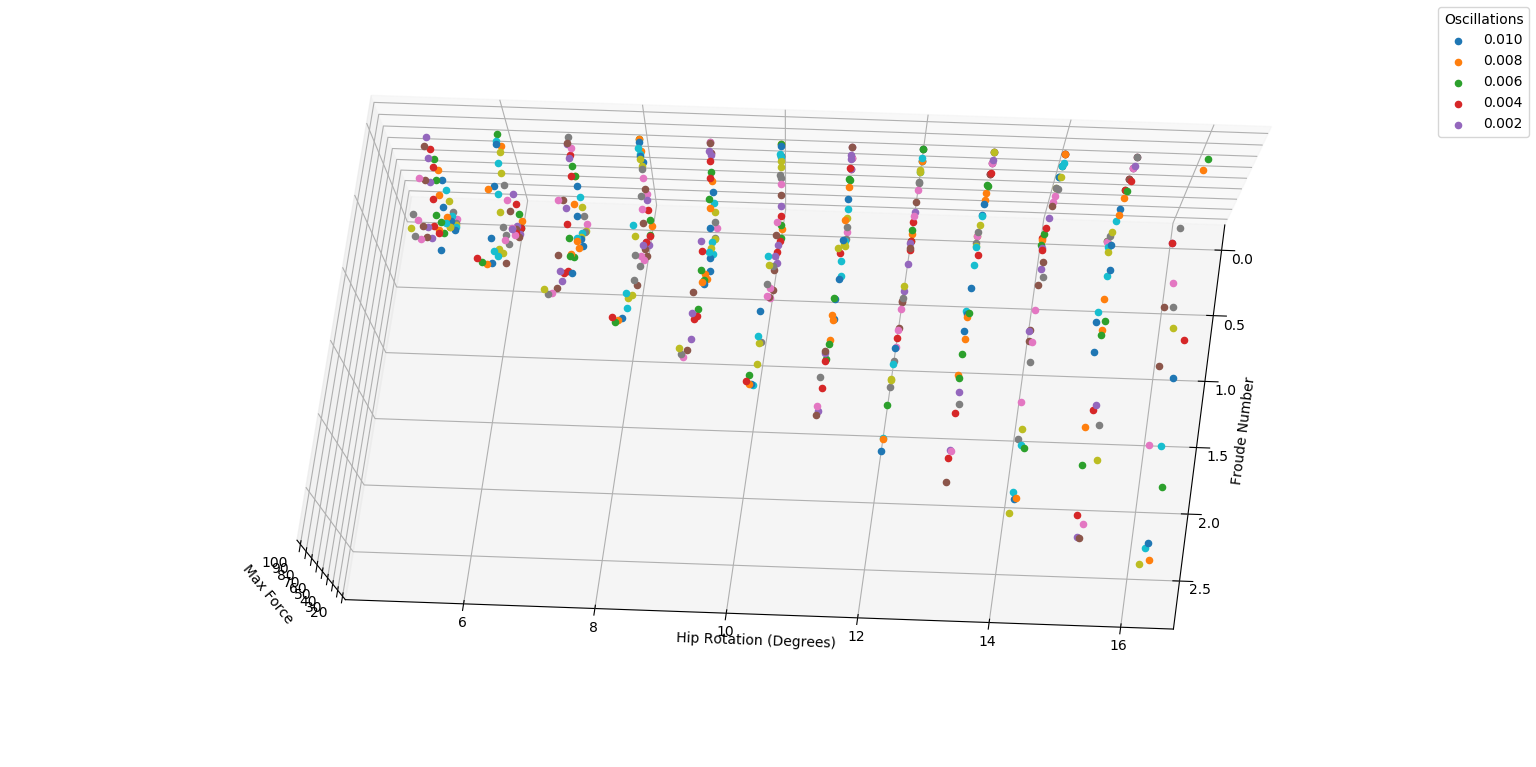
\includegraphics[width=1\textwidth]{figures/forcerotationfroude2.png}
    \label{froudenumbervsangle}
    \caption{All variation of experiments shown on 3D gragh, view 2}
\end{figure}

\begin{figure}[h!]
  \centering
  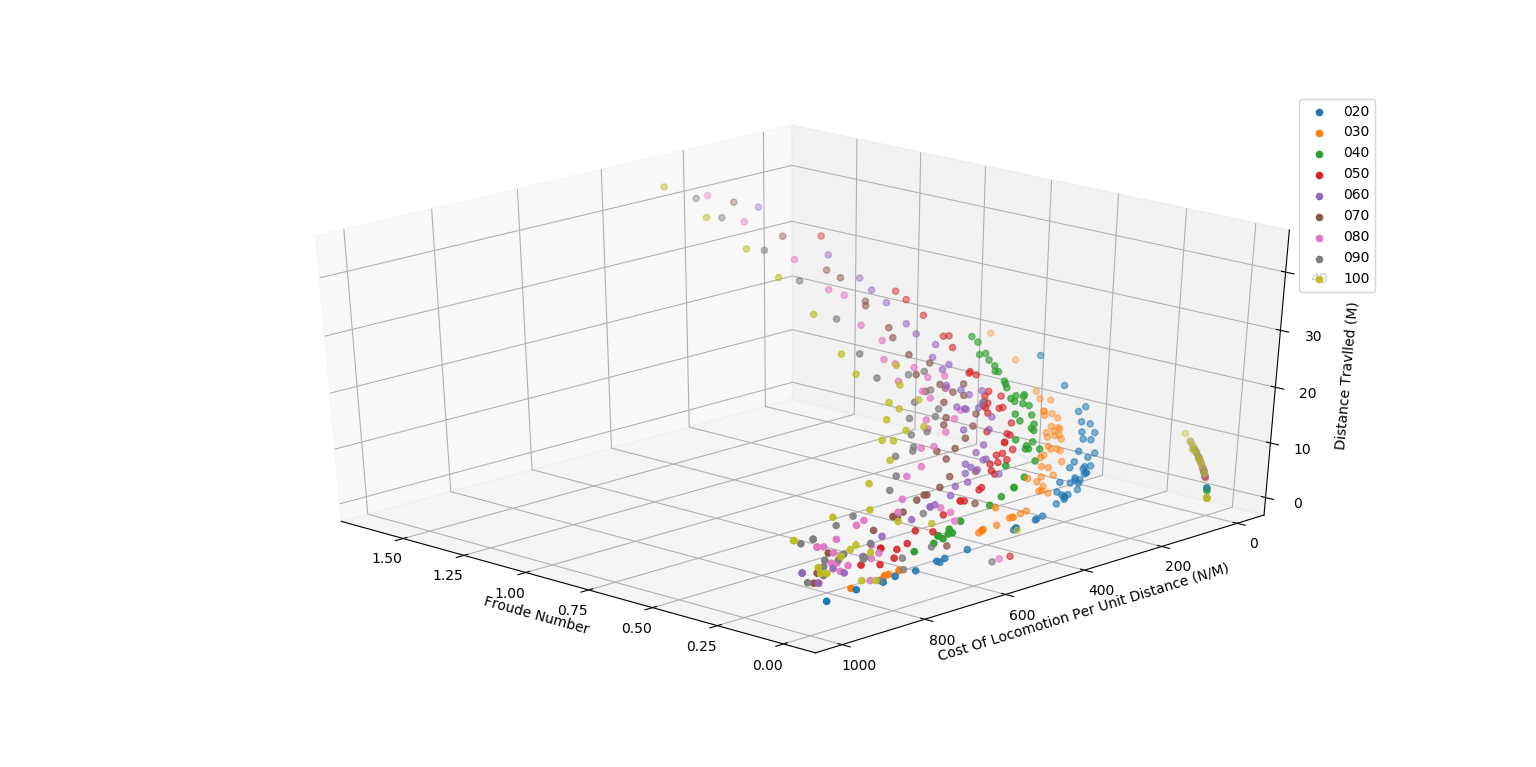
\includegraphics[width=1\textwidth]{figures/3dgraph.png} 
  \caption{Cost Of Locomotion against force applied, distance travelled on Y.}
  \label{3dgraph1}
\end{figure}

\begin{figure}[h!]
  \centering
  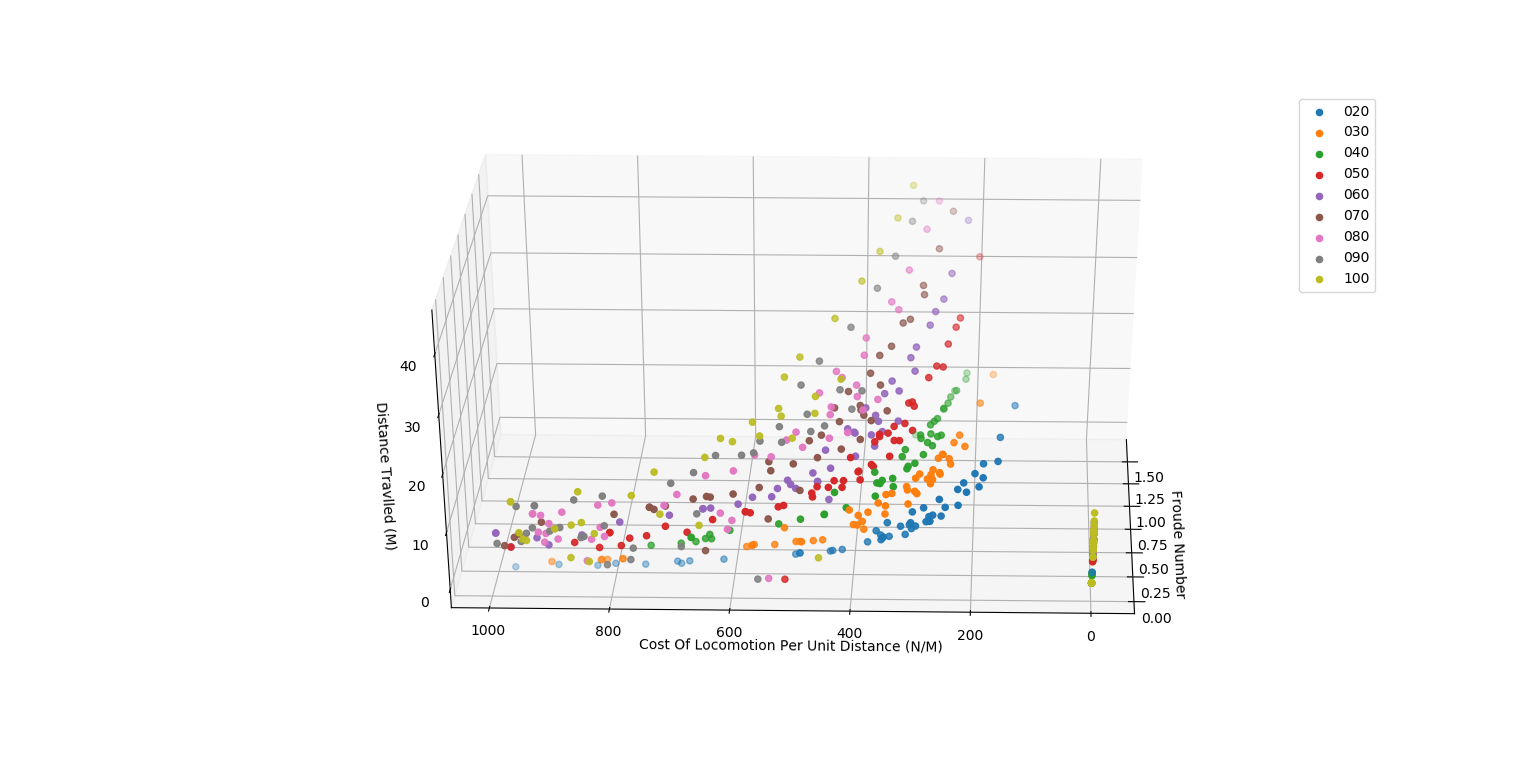
\includegraphics[width=1\textwidth]{figures/3dgraph2.png}
  \caption{Cost Of Locomotion against force applied, distance travelled on Y view 2.}
  \label{3dgraph2}
\end{figure}

\begin{figure}[h!]
  \centering
  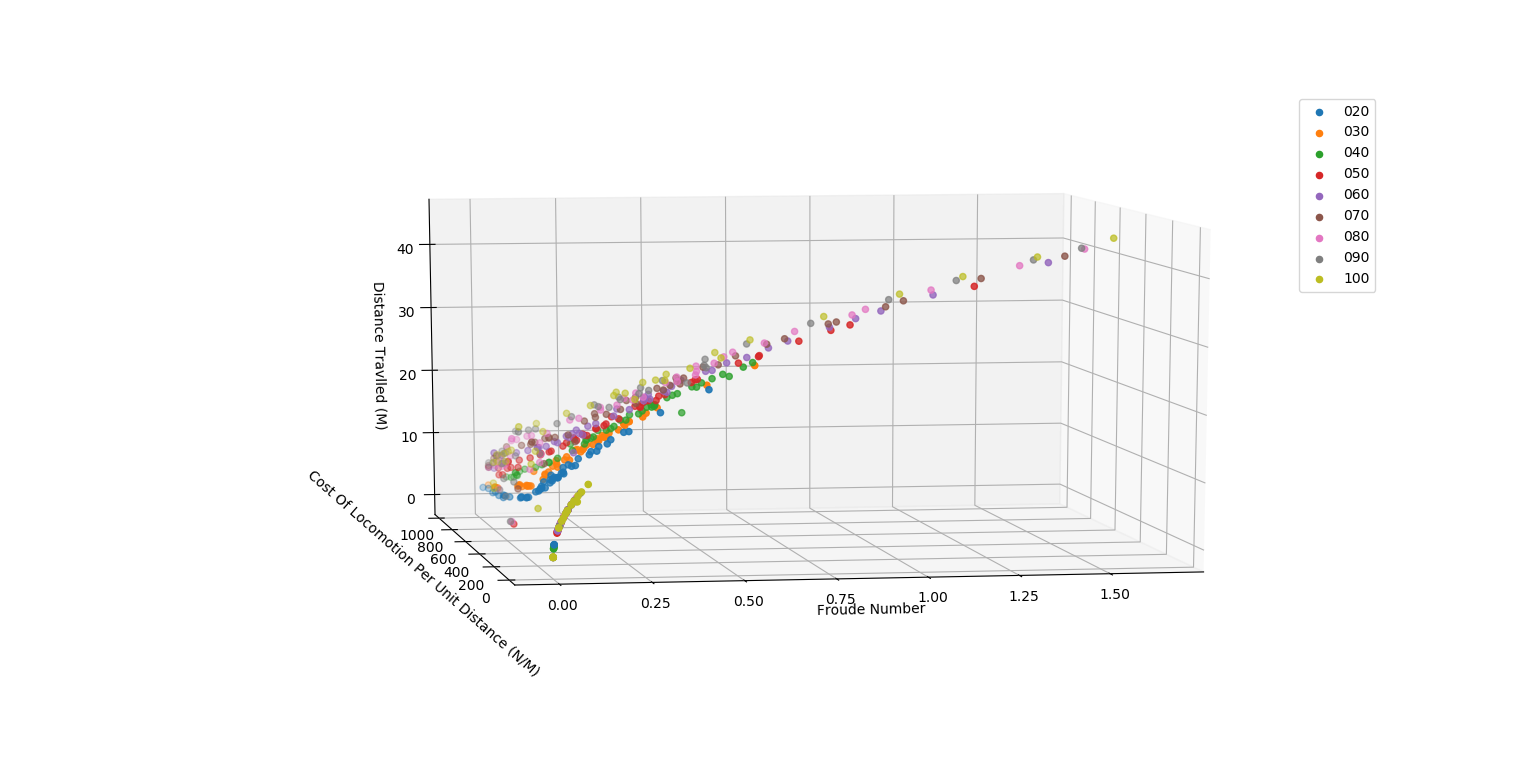
\includegraphics[width=1\textwidth]{figures/3dgraph3.png}
  \caption{Cost Of Locomotion against force applied, distance travelled on Y view 3.}
  \label{3dgraph2}
\end{figure}

\end{appendices}

\end{document}
